\documentclass[11pt]{article}
\usepackage[utf8]{inputenc}
\usepackage[T1]{fontenc}
\usepackage{lmodern}
\usepackage[letterpaper,margin=2.2cm]{geometry}
\usepackage{graphicx}
\usepackage{booktabs}
\usepackage{array}
\usepackage{longtable}
\usepackage{float}
\usepackage{xcolor}
\usepackage{hyperref}
\usepackage{amsmath}
\hypersetup{colorlinks=true,linkcolor=blue!55!black,urlcolor=blue!65!black,citecolor=teal!55!black}
\graphicspath{{../outputs/figures/}}
\definecolor{navy}{HTML}{102A43}
\definecolor{teal}{HTML}{0F9D91}
\definecolor{soft}{HTML}{F1F5F9}
\newcommand{\repo}{\href{https://github.com/DanielBarillasM/Laboratorio-6.-Analitica-de-Redes-Sociales_Grupo-1_DS_Sec-10}{Repositorio de GitHub}}
\setlength{\parindent}{0pt}
\setlength{\parskip}{0.6em}

\begin{document}

\hypersetup{pageanchor=false}
\begin{titlepage}
\pagecolor{navy}\color{white}
\centering
\vspace*{1.4cm}
{\Large Universidad del Valle de Guatemala\par}
\vspace{0.4cm}
{\large Facultad de Ingeniería\par}
{\large CC3084 -- Data Science, Sección 10\par}
\vfill
{\Huge\bfseries Laboratorio 6\par}
\vspace{0.3cm}
{\LARGE Analítica de Redes Sociales\par}
\vspace{0.9cm}
{\Large\color{teal!25!white}Documento final -- 100\%\par}
\vfill
{\large Grupo 1\par}
\vspace{0.5cm}
\begin{tabular}{rl}
Jorge Gabriel Palacios Sales & 231385\\
Pablo Daniel Barillas Moreno & 22193\\
Roberto Emiliano Otoniel & 23968\\
\end{tabular}
\vfill
{\large Segundo semestre de 2026\par}
\end{titlepage}
\nopagecolor\color{black}
\hypersetup{pageanchor=true}
\pagenumbering{arabic}

\tableofcontents
\newpage

\section{Resumen ejecutivo}

Se analizaron 293 videos, 97 canales, 406 comentarios y 332 autores de una muestra obtenida de YouTube. El flujo reproducible carga archivos CSV o Excel, normaliza identificadores, limpia texto en español, integra las dos tablas, describe participación y construye la red autor--video, sus proyecciones autor--autor y video--video, métricas topológicas, comunidades (Louvain ponderado), centralidades, participantes puente/articuladores y análisis de sentimiento con RoBERTuito. Este documento cierra los diez ejercicios del laboratorio.

El 100\% de los comentarios se asoció con un video. La participación está fuertemente concentrada: el video \emph{Qué rico come tu diputado} contiene 161 comentarios (39.7\% del total), los cinco videos principales reúnen 75.4\%, y el canal Quorum concentra 256 comentarios (63.1\%). La red bipartita completa contiene 625 nodos y 343 aristas; conserva 274 videos aislados para representar la cobertura real. La proyección de autores presenta una componente principal con 83.1\% de los autores y diez comunidades con modularidad 0.395.

La entrega final cubre los diez ejercicios y los 100 puntos trazables de la rúbrica. Cada criterio cuenta con evidencia reproducible en el notebook, las tablas, las figuras y este informe.

\section{Alcance de la entrega final}

El trabajo comprende calidad y preprocesamiento, análisis exploratorio, construcción de la red bipartita, proyecciones, topología, comunidades, centralidades, participantes puente, análisis de contenido y sentimiento, interpretación y conclusiones. La tabla resume la correspondencia entre la rúbrica y la evidencia producida.

\begin{table}[H]
\centering
\caption{Cobertura final de la rúbrica.}
\begin{tabular}{p{0.53\textwidth}rrl}
\toprule
Criterio & Total & Cubierto & Estado\\
\midrule
Calidad, limpieza y preprocesamiento & 18 & 18 & Completo\\
Análisis exploratorio & 18 & 18 & Completo\\
Red bipartita autor--video & 10 & 10 & Completo\\
Proyecciones & 8 & 8 & Completo\\
Topología y fragmentación & 12 & 12 & Completo\\
Comunidades & 10 & 10 & Completo\\
Centralidad y participantes puente & 7 & 7 & Completo\\
Contenido y sentimiento & 5 & 5 & Completo\\
Interpretación y conclusiones finales & 12 & 12 & Completo\\
\midrule
Total & 100 & 100 & Entrega final\\
\bottomrule
\end{tabular}
\end{table}

\section{Datos, unidades e integración}

Cada fila de videos representa un video y su llave primaria es \texttt{video\_id}; cada fila de comentarios representa un comentario principal y su llave es \texttt{comment\_id}. \texttt{channel\_id} identifica el canal propietario, mientras \texttt{author\_channel\_id} identifica al autor del comentario. Los nombres y handles se usan únicamente como etiquetas visibles.

Se utilizaron los archivos originales \texttt{youtube\_videos.csv} y \texttt{youtube\_comments.csv} solicitados por la guía. Ambos fueron verificados como CSV reales. Los 293 identificadores de video están completos y son únicos, por lo que no fue necesario reconstruirlos. El cargador conserva detección por firma binaria y recuperación auditable desde \texttt{video\_url} como controles defensivos ante futuras exportaciones en Excel.

\begin{table}[H]
\centering
\caption{Dimensiones e integración.}
\begin{tabular}{lr}
\toprule
Indicador & Valor\\
\midrule
Videos & 293\\
Canales únicos & 97\\
Comentarios & 406\\
Autores únicos & 332\\
Videos con comentarios & 19\\
Videos sin comentarios & 274\\
IDs de video recuperados & 0\\
Comentarios asociados & 406 (100\%)\\
\bottomrule
\end{tabular}
\end{table}

La relación canal--video es de uno a muchos en la muestra. Un autor puede comentar varios videos y un video puede recibir comentarios de varios autores. \texttt{source\_query} describe cómo se obtuvo el registro, no necesariamente su tema definitivo.

\section{Calidad, limpieza y preprocesamiento}

Se evaluaron dimensiones, tipos, valores faltantes, duplicados, constantes, atípicos y consistencia de IDs, nombres y handles. No hay duplicados completos y las llaves primarias son completas y únicas. \texttt{viewer\_rating} está vacío en los 406 comentarios y \texttt{is\_pinned} es constante; el primero se excluye y el segundo se conserva solo para auditoría. Las fechas relativas no se transforman en fechas exactas.

Los espacios de \texttt{like\_count\_text} se interpretan como cero y el parser contempla separadores y sufijos K, M, \emph{mil} y \emph{millones}. \texttt{reply\_count} se conserva como conteo descriptivo: no identifica autores de respuesta y, por tanto, nunca origina aristas entre usuarios.

Para cada comentario se conserva \texttt{texto\_original} y se produce \texttt{texto\_limpio}. La limpieza decodifica HTML, convierte a minúsculas, elimina URL y menciones, retiene la palabra de los hashtags sin el símbolo, extrae palabras Unicode, elimina números, puntuación, emojis y una lista explícita de stopwords en español. Los emojis permanecen en el original para el futuro análisis de sentimiento. No se aplicó lematización en esta fase porque hacerlo sin un modelo morfosintáctico validado para español podría deformar nombres y términos temáticos.

\begin{table}[H]
\centering
\caption{Efecto cuantificado de la limpieza textual.}
\begin{tabular}{lr}
\toprule
Métrica & Valor\\
\midrule
Registros de entrada & 406\\
Textos modificados & 403\\
Textos vacíos antes & 0\\
Textos vacíos después & 6\\
Duplicados textuales antes & 2\\
Duplicados textuales después & 11\\
Registros eliminados & 0\\
\bottomrule
\end{tabular}
\end{table}

Los textos vacíos posteriores no se eliminan: mantienen la trazabilidad del comentario y sus atributos de red, pero se excluyen naturalmente de frecuencias léxicas.

\section{Análisis exploratorio}

\begin{figure}[H]
\centering
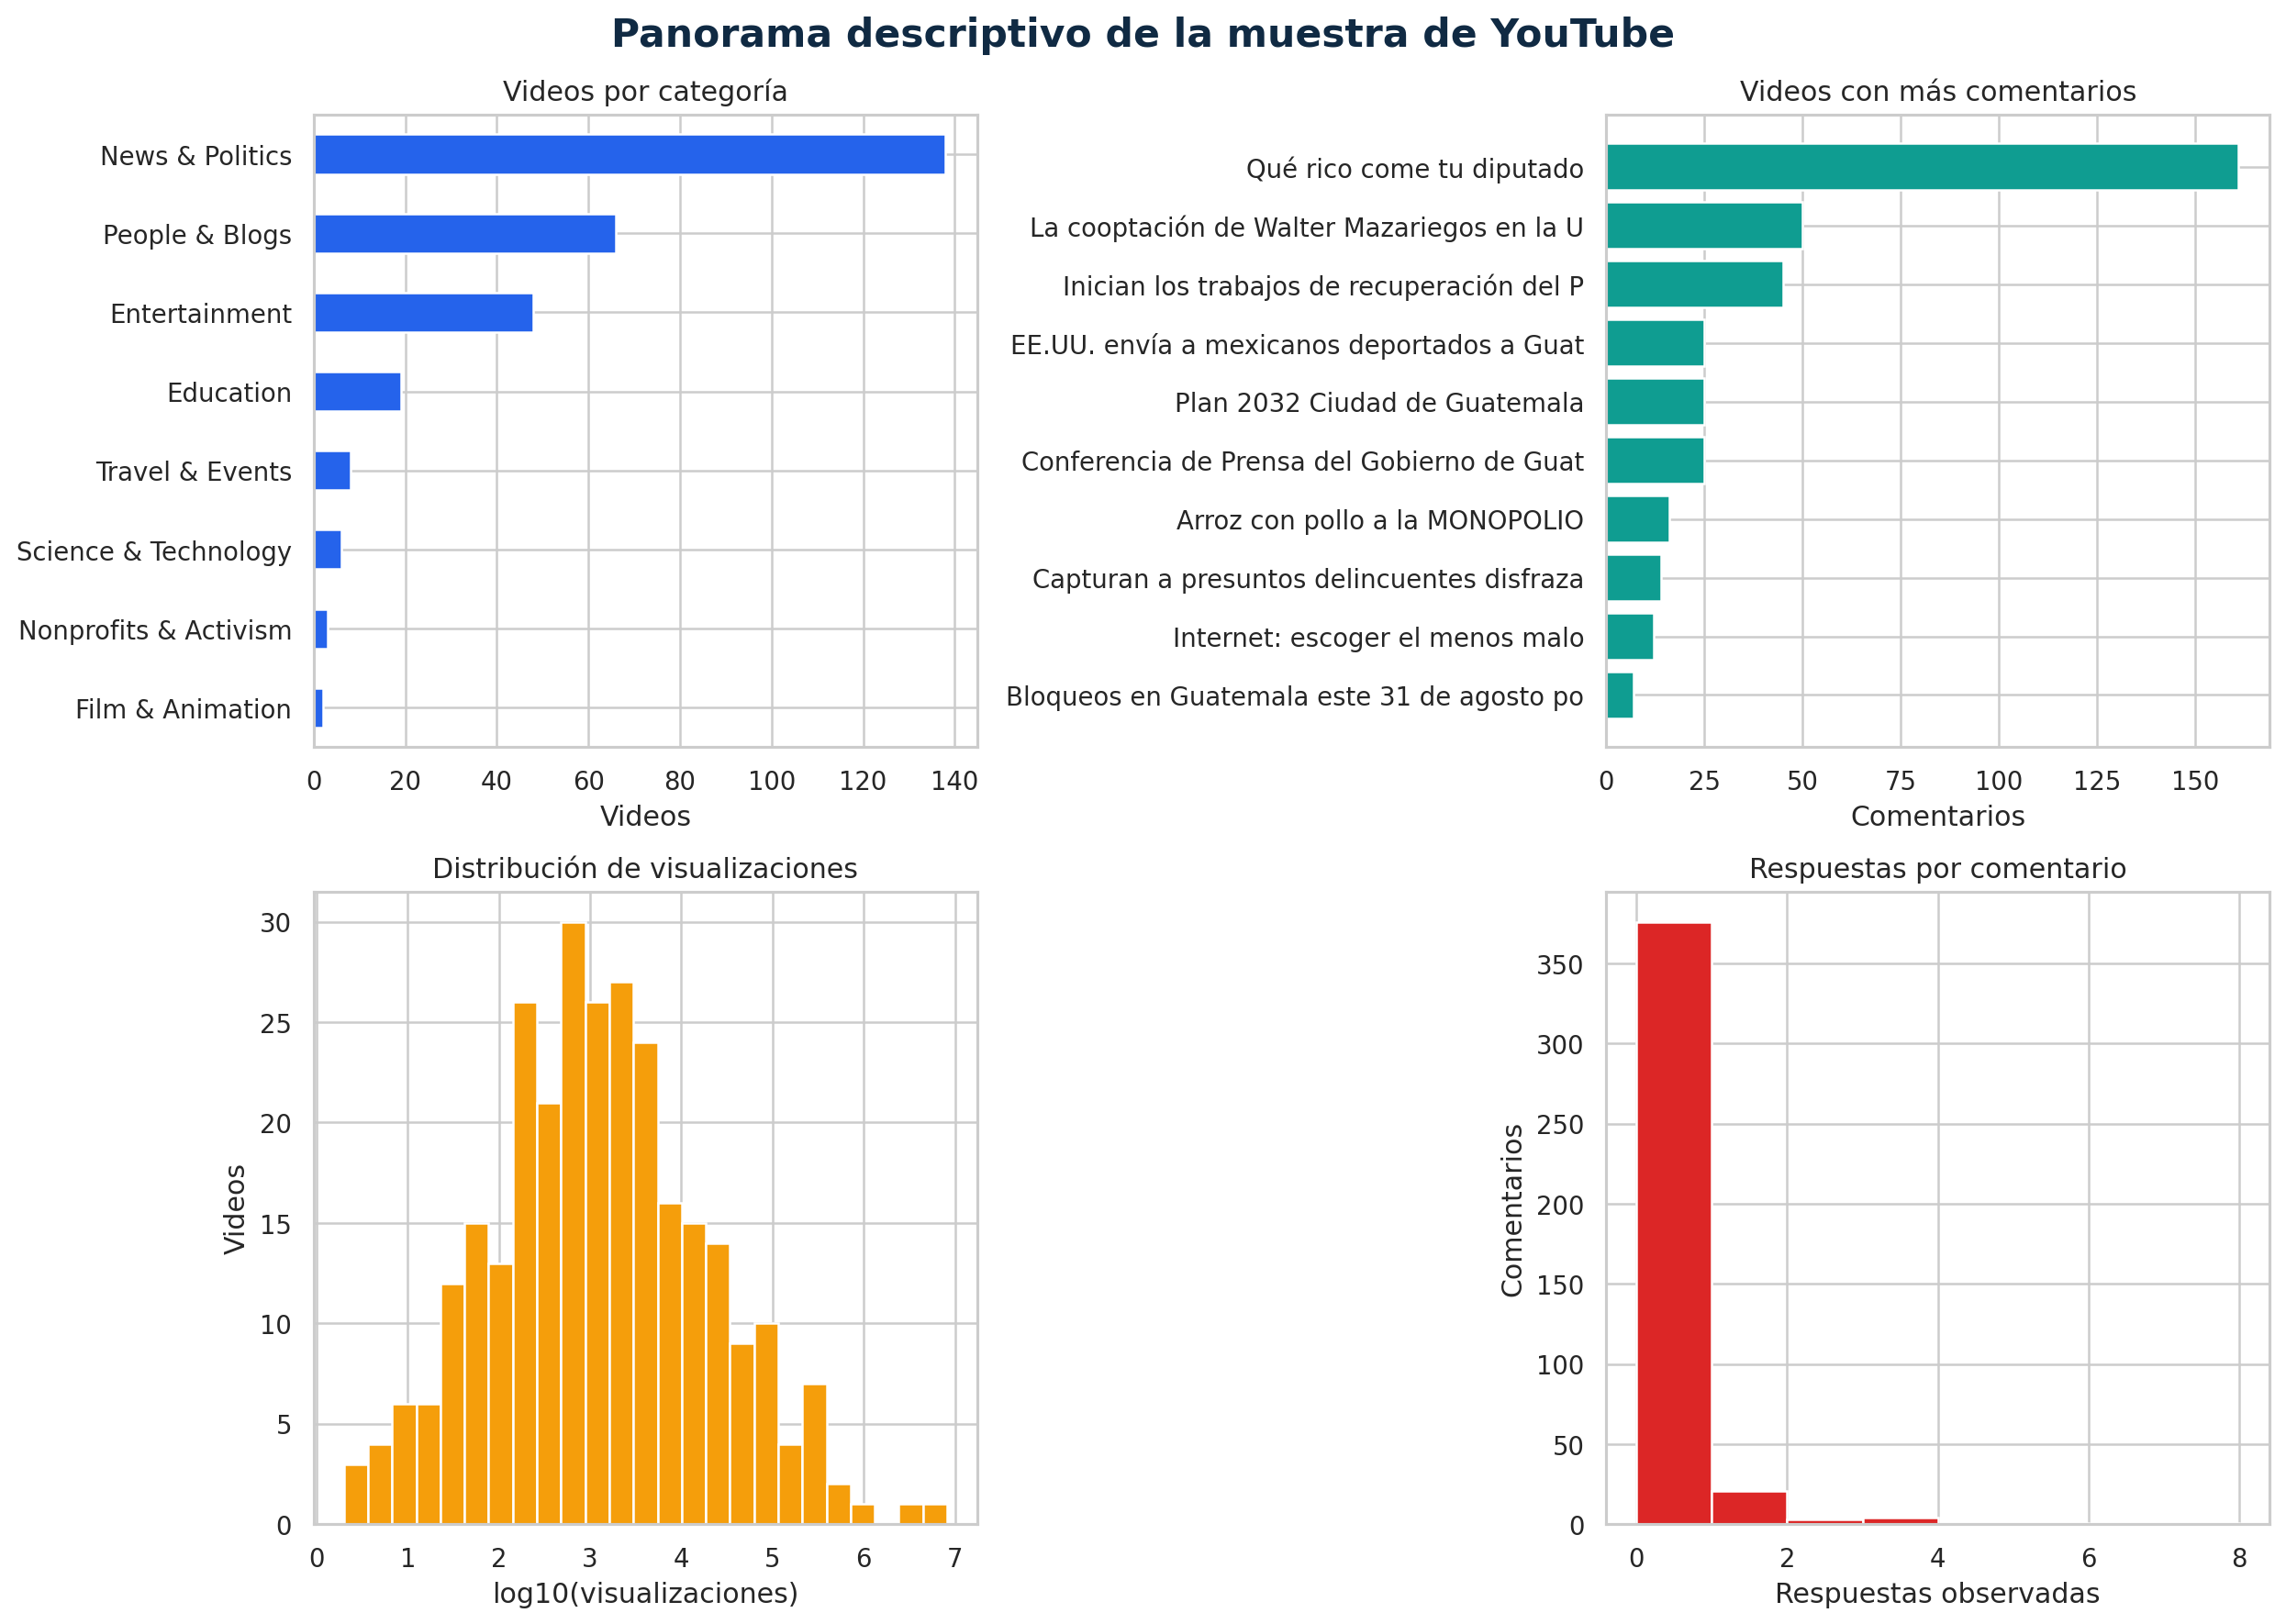
\includegraphics[width=0.98\textwidth]{eda_panorama.png}
\caption{Categorías, participación, visualizaciones y respuestas en la muestra.}
\label{fig:eda}
\end{figure}

La categoría dominante es \emph{News \& Politics}. Las visualizaciones son marcadamente asimétricas: la mediana es 1,175, mientras el máximo supera 8.19 millones. Esta diferencia justifica escalas logarítmicas y medidas robustas. La mayoría de comentarios no recibió respuestas y la cobertura se concentra en solo 19 videos.

\begin{figure}[H]
\centering
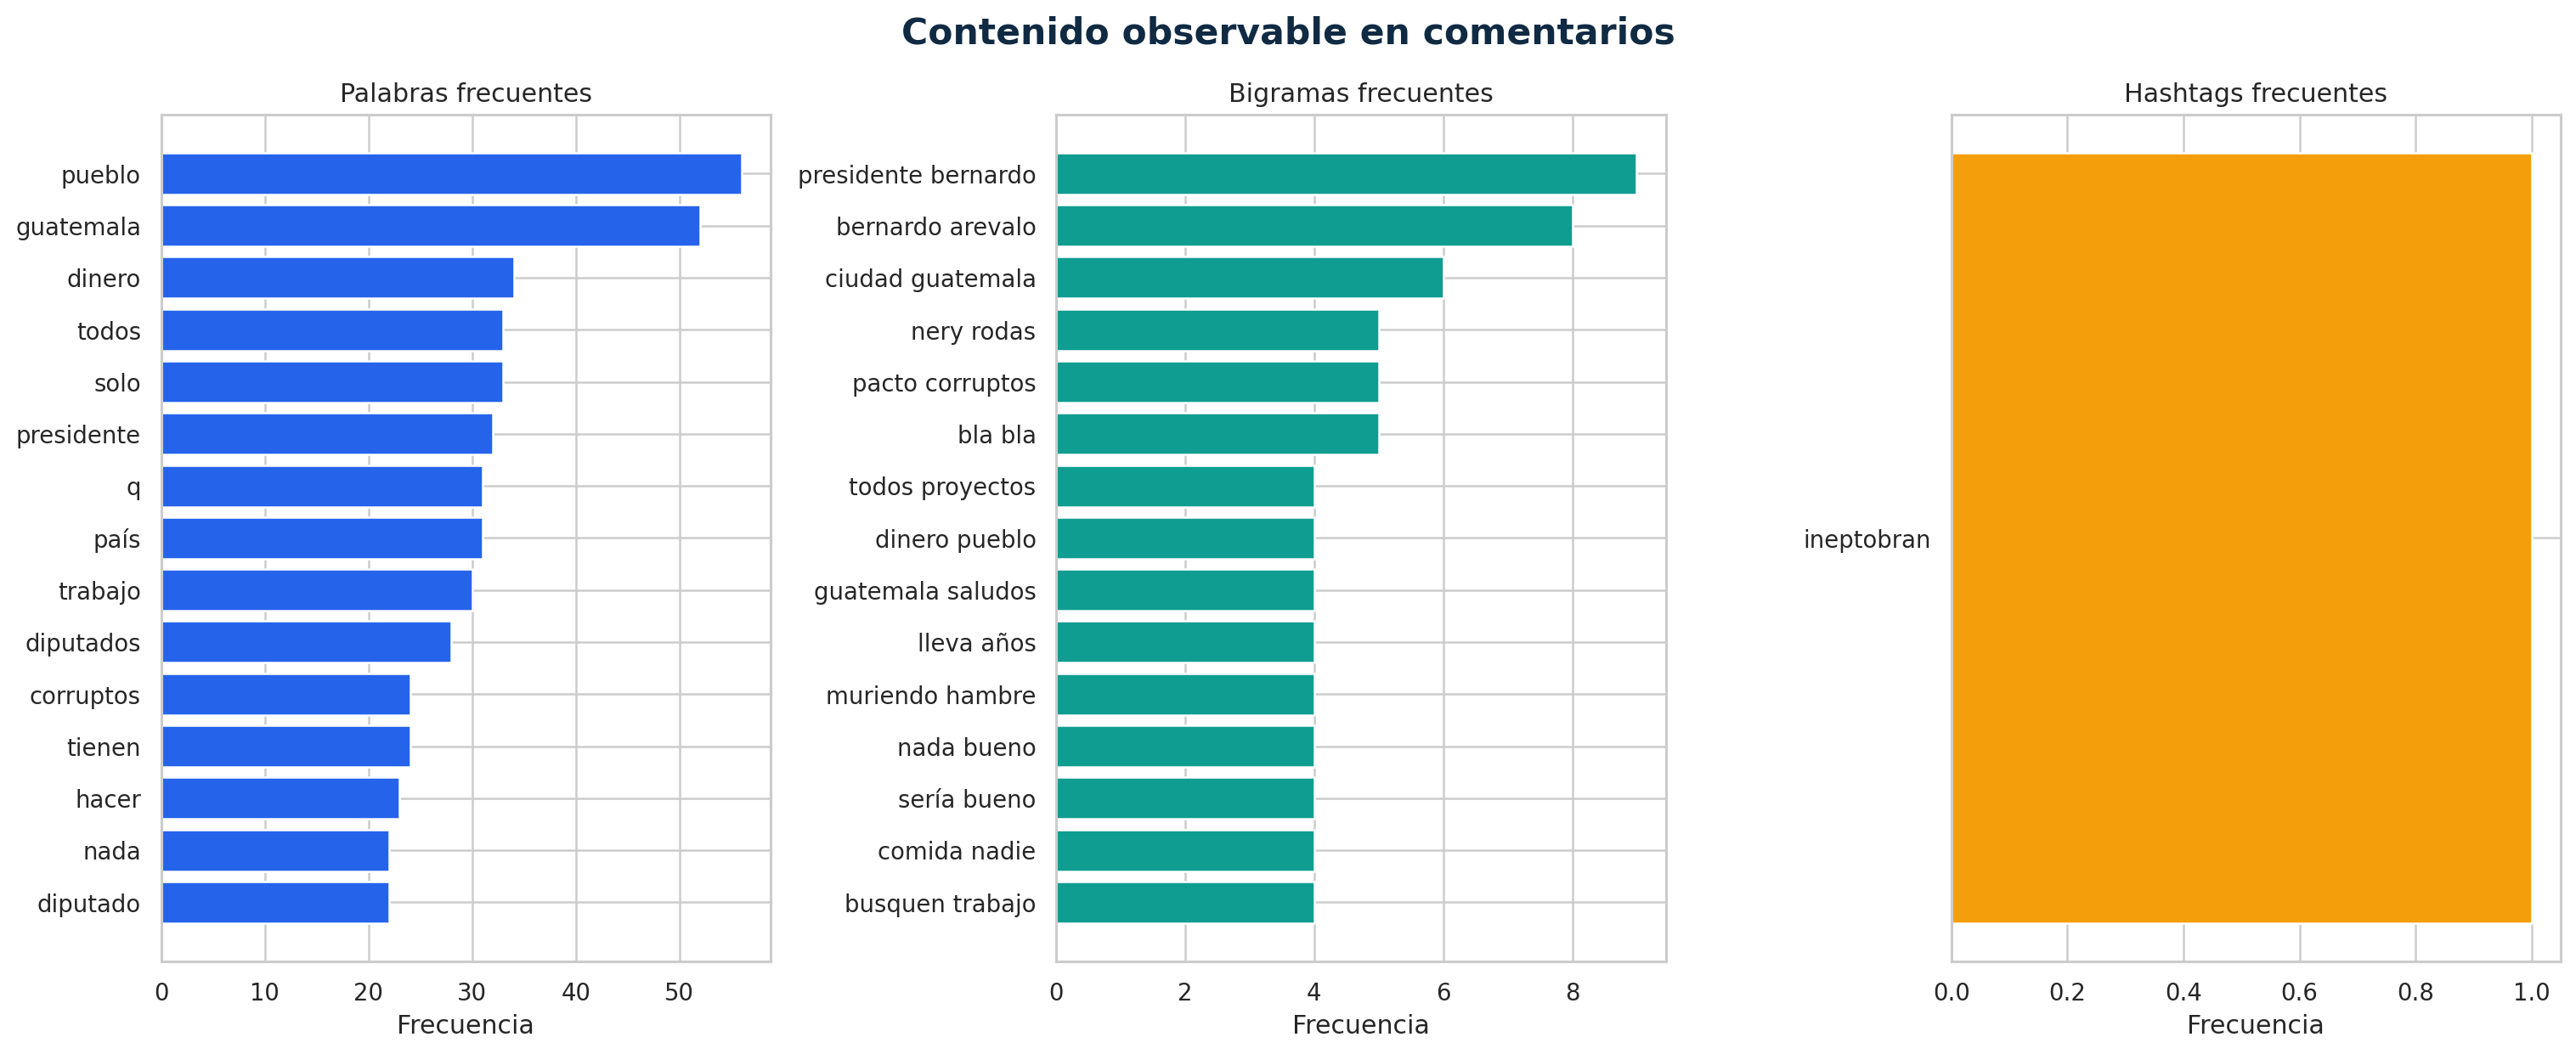
\includegraphics[width=0.98\textwidth]{frecuencias_contenido.png}
\caption{Palabras, bigramas y hashtags frecuentes después de la limpieza.}
\label{fig:texto}
\end{figure}

Las frecuencias reflejan principalmente conversación política, asuntos públicos, Guatemala, gobierno, universidad y condiciones sociales. Se reportan tanto frecuencias como probabilidades relativas en los CSV, para que los resultados sean comparables y reconstruibles. Una nube de palabras no se usó como sustituto de estas comparaciones cuantitativas.

\subsection{Concentración de participación}

\begin{figure}[H]
\centering
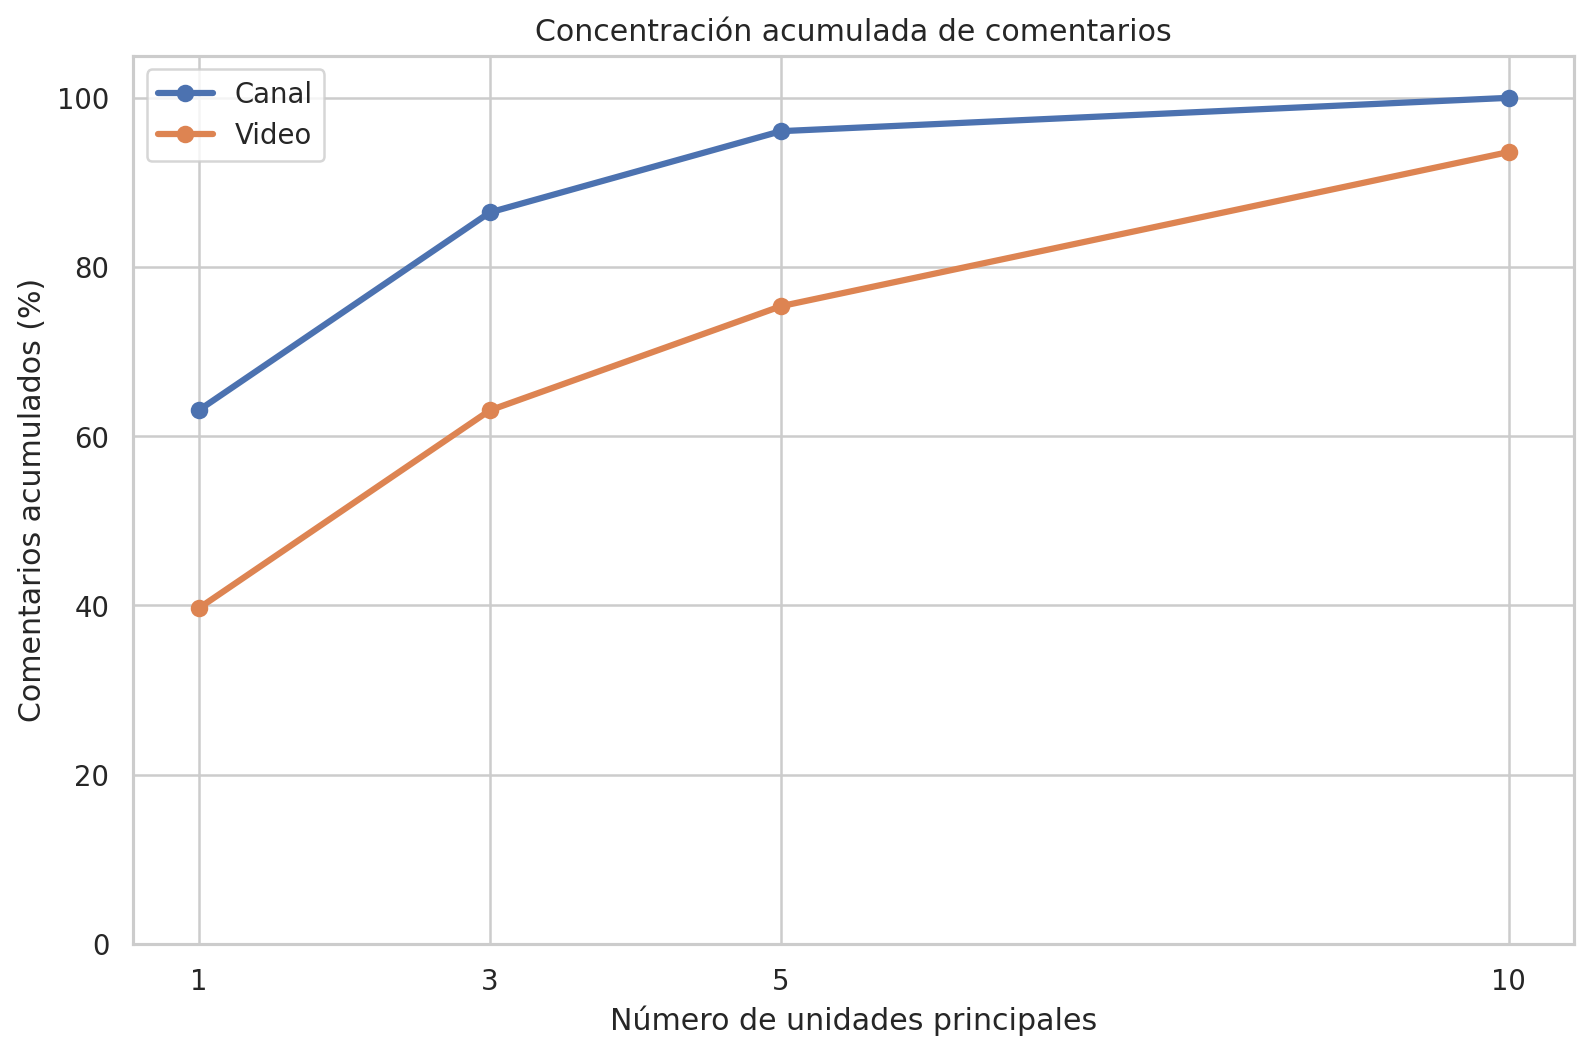
\includegraphics[width=0.78\textwidth]{concentracion_participacion.png}
\caption{Participación acumulada en las unidades más activas.}
\label{fig:concentracion}
\end{figure}

El video principal reúne 39.7\% de los comentarios; los tres primeros, 63.1\%; los cinco primeros, 75.4\%; y los diez primeros, 93.6\%. Quorum concentra 63.1\% de los comentarios, y los tres canales principales 86.5\%. Por ello, las propiedades observadas describen sobre todo unos pocos contenidos activos.

\subsection{Visibilidad y participación}

\begin{figure}[H]
\centering
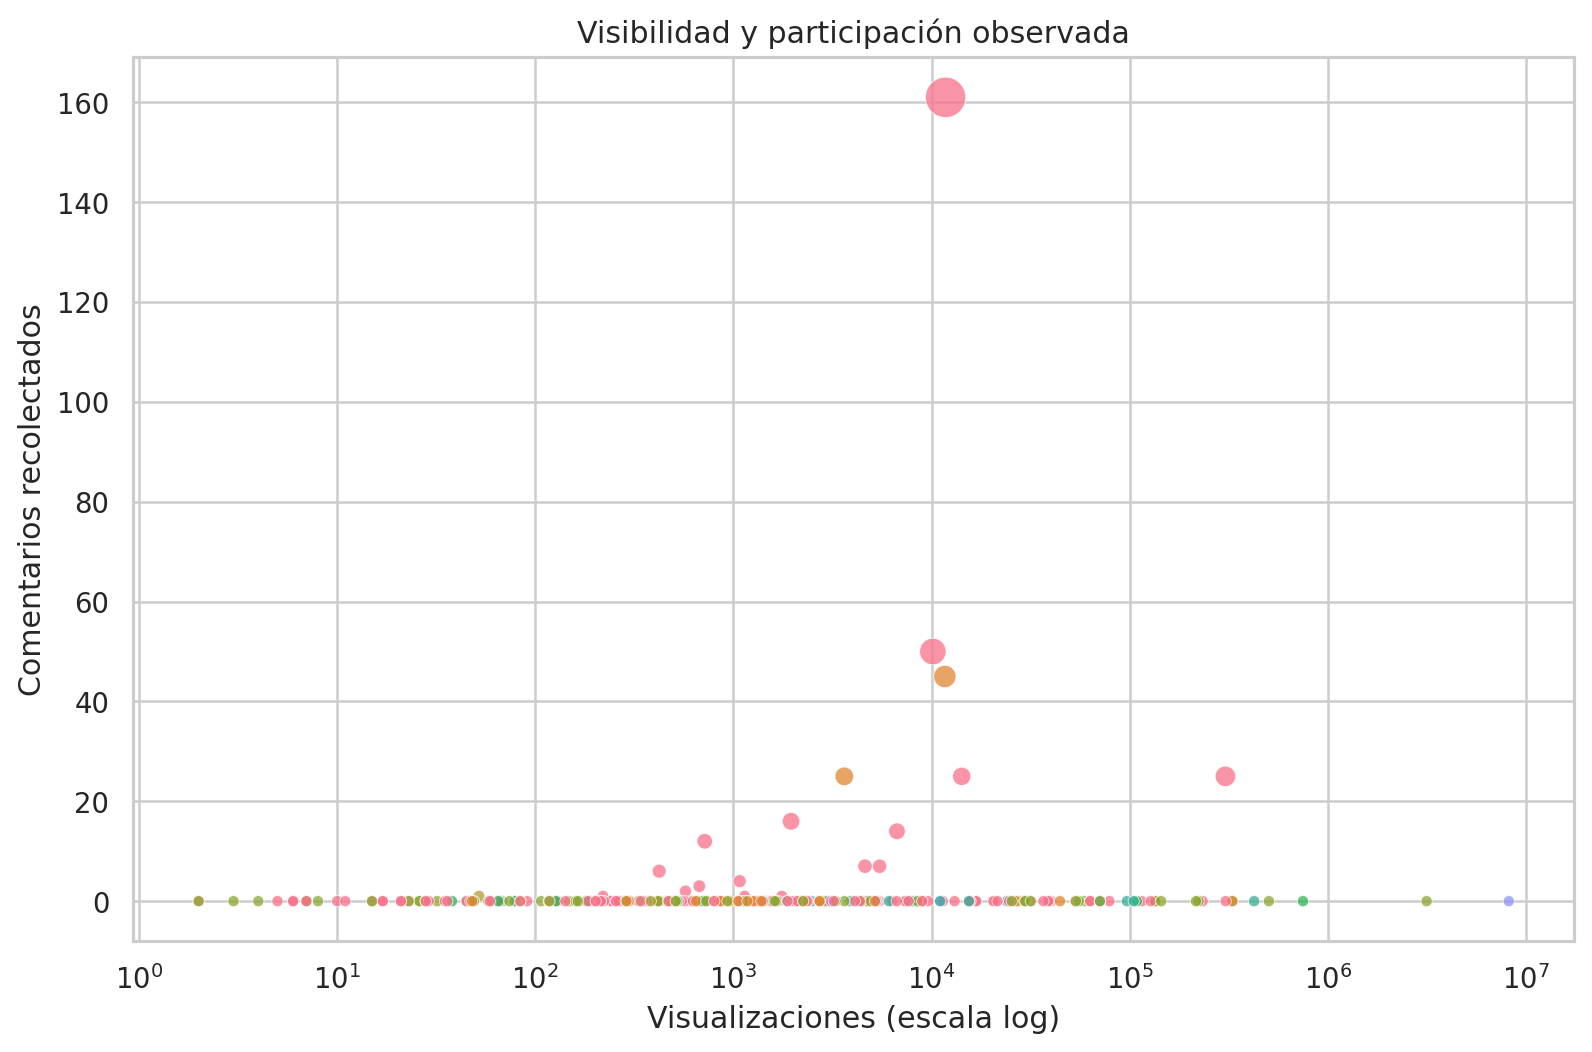
\includegraphics[width=0.78\textwidth]{visibilidad_vs_participacion.png}
\caption{Visualizaciones frente a comentarios recolectados.}
\label{fig:visibilidad}
\end{figure}

En los 293 videos, Spearman produce $\rho=0.080$ ($p=0.170$), asociación débil y no significativa. Al restringir a los 19 videos con comentarios, $\rho=0.811$ ($p<0.001$). La diferencia no debe interpretarse como contradicción: la primera estimación incorpora 274 ceros estructurales causados por cobertura, mientras la segunda sufre selección. Las visualizaciones y comentarios también fueron observados en un momento específico y no miden exactamente el mismo proceso.

\section{Preguntas obligatorias y adicionales}

\begin{enumerate}
  \item \textbf{¿Qué videos y canales concentran participación?} \emph{Qué rico come tu diputado} lidera con 161 comentarios; Quorum lidera con 256. Los cinco videos principales reúnen 75.4\%.
  \item \textbf{¿Existen audiencias compartidas?} Sí, en el sentido limitado de coparticipación: la proyección video--video contiene 11 pares unidos por autores compartidos y la proyección autor--autor 10,732 pares.
  \item \textbf{¿Qué autores funcionan como puentes?} Nueve autores participaron en más de un video, siete son puntos de articulación y 12 de los 25 nodos candidatos evaluados fragmentan la red al removerse. @virgiliogarcia3039 produce el mayor cambio: la componente principal de autores cae 22.5\%.
  \item \textbf{¿Qué temas y sentimientos caracterizan comunidades?} Las comunidades principales se relacionan con diputados y gasto público, gobierno y país, y USAC/corrupción. RoBERTuito clasifica como negativo el 61.3\% del corpus; la distribución por comunidad se reporta con un mínimo de cinco comentarios.
  \item \textbf{¿Coinciden visibilidad y participación?} No de forma general en la muestra completa: $\rho=0.080$. La asociación alta entre videos cubiertos no elimina el sesgo de selección.
  \item \textbf{¿Qué limita las conclusiones?} Consultas de búsqueda, fechas relativas, conteos instantáneos, ausencia de respuestas identificadas, 19 videos cubiertos y concentración extrema.
\end{enumerate}

Preguntas adicionales: (1) ¿qué tan recurrente es la audiencia entre videos?, respondida mediante el número de autores con más de un video; (2) ¿cuántos comentarios presentan al menos una respuesta?, sin inferir quién respondió; (3) ¿cómo se distribuye la conversación según \texttt{source\_group}?; y (4) ¿cuántos comentarios no muestran likes después de normalizar espacios? Las respuestas exactas se conservan en \texttt{preguntas\_adicionales.csv}.

\section{Red bipartita autor--video}

Se construyó una red no dirigida con autores y videos como tipos de nodo. Una arista existe cuando un autor comentó un video; su peso es el número de comentarios de ese autor en ese video. La arista no demuestra amistad, conversación directa, acuerdo ni aprobación.

\begin{figure}[H]
\centering
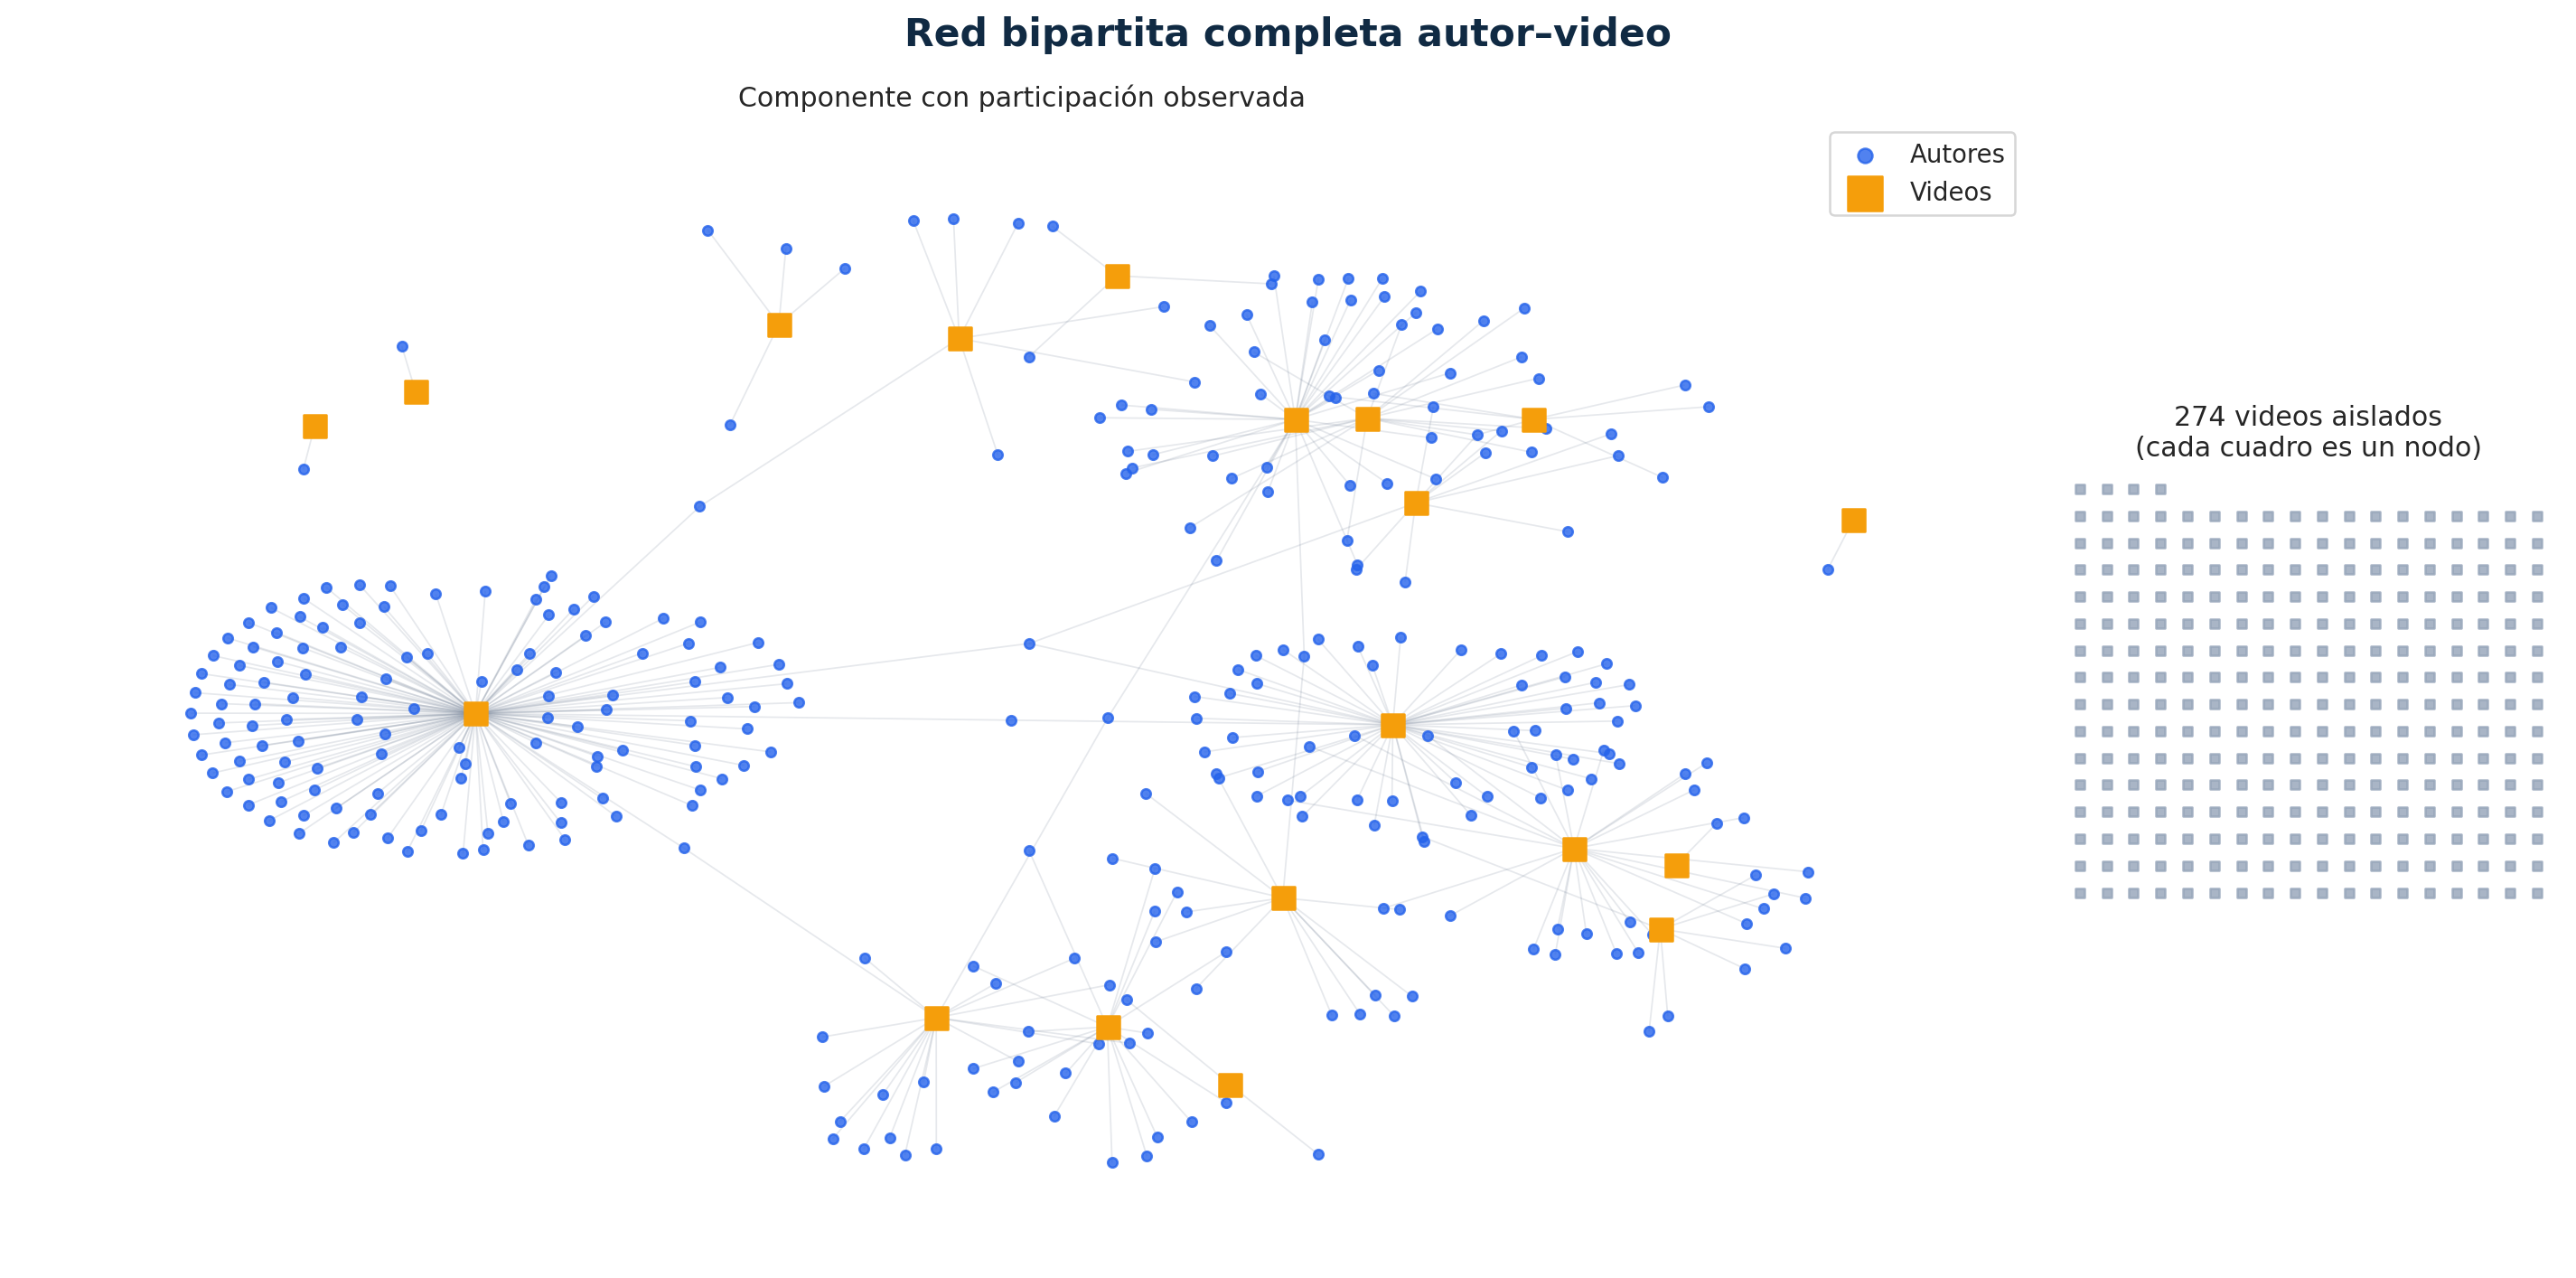
\includegraphics[width=0.98\textwidth]{red_bipartita_completa.png}
\caption{Red bipartita. La vista estructural muestra nodos activos y el panel conserva el conteo de aislados.}
\label{fig:bipartita}
\end{figure}

La tabla de nodos contiene tipo, identificador y atributos relevantes. La tabla de aristas conserva origen, destino, peso y significado. Los 274 videos sin comentarios permanecen como aislados; no se eliminaron para mejorar la apariencia.

\section{Proyecciones}

\begin{figure}[H]
\centering
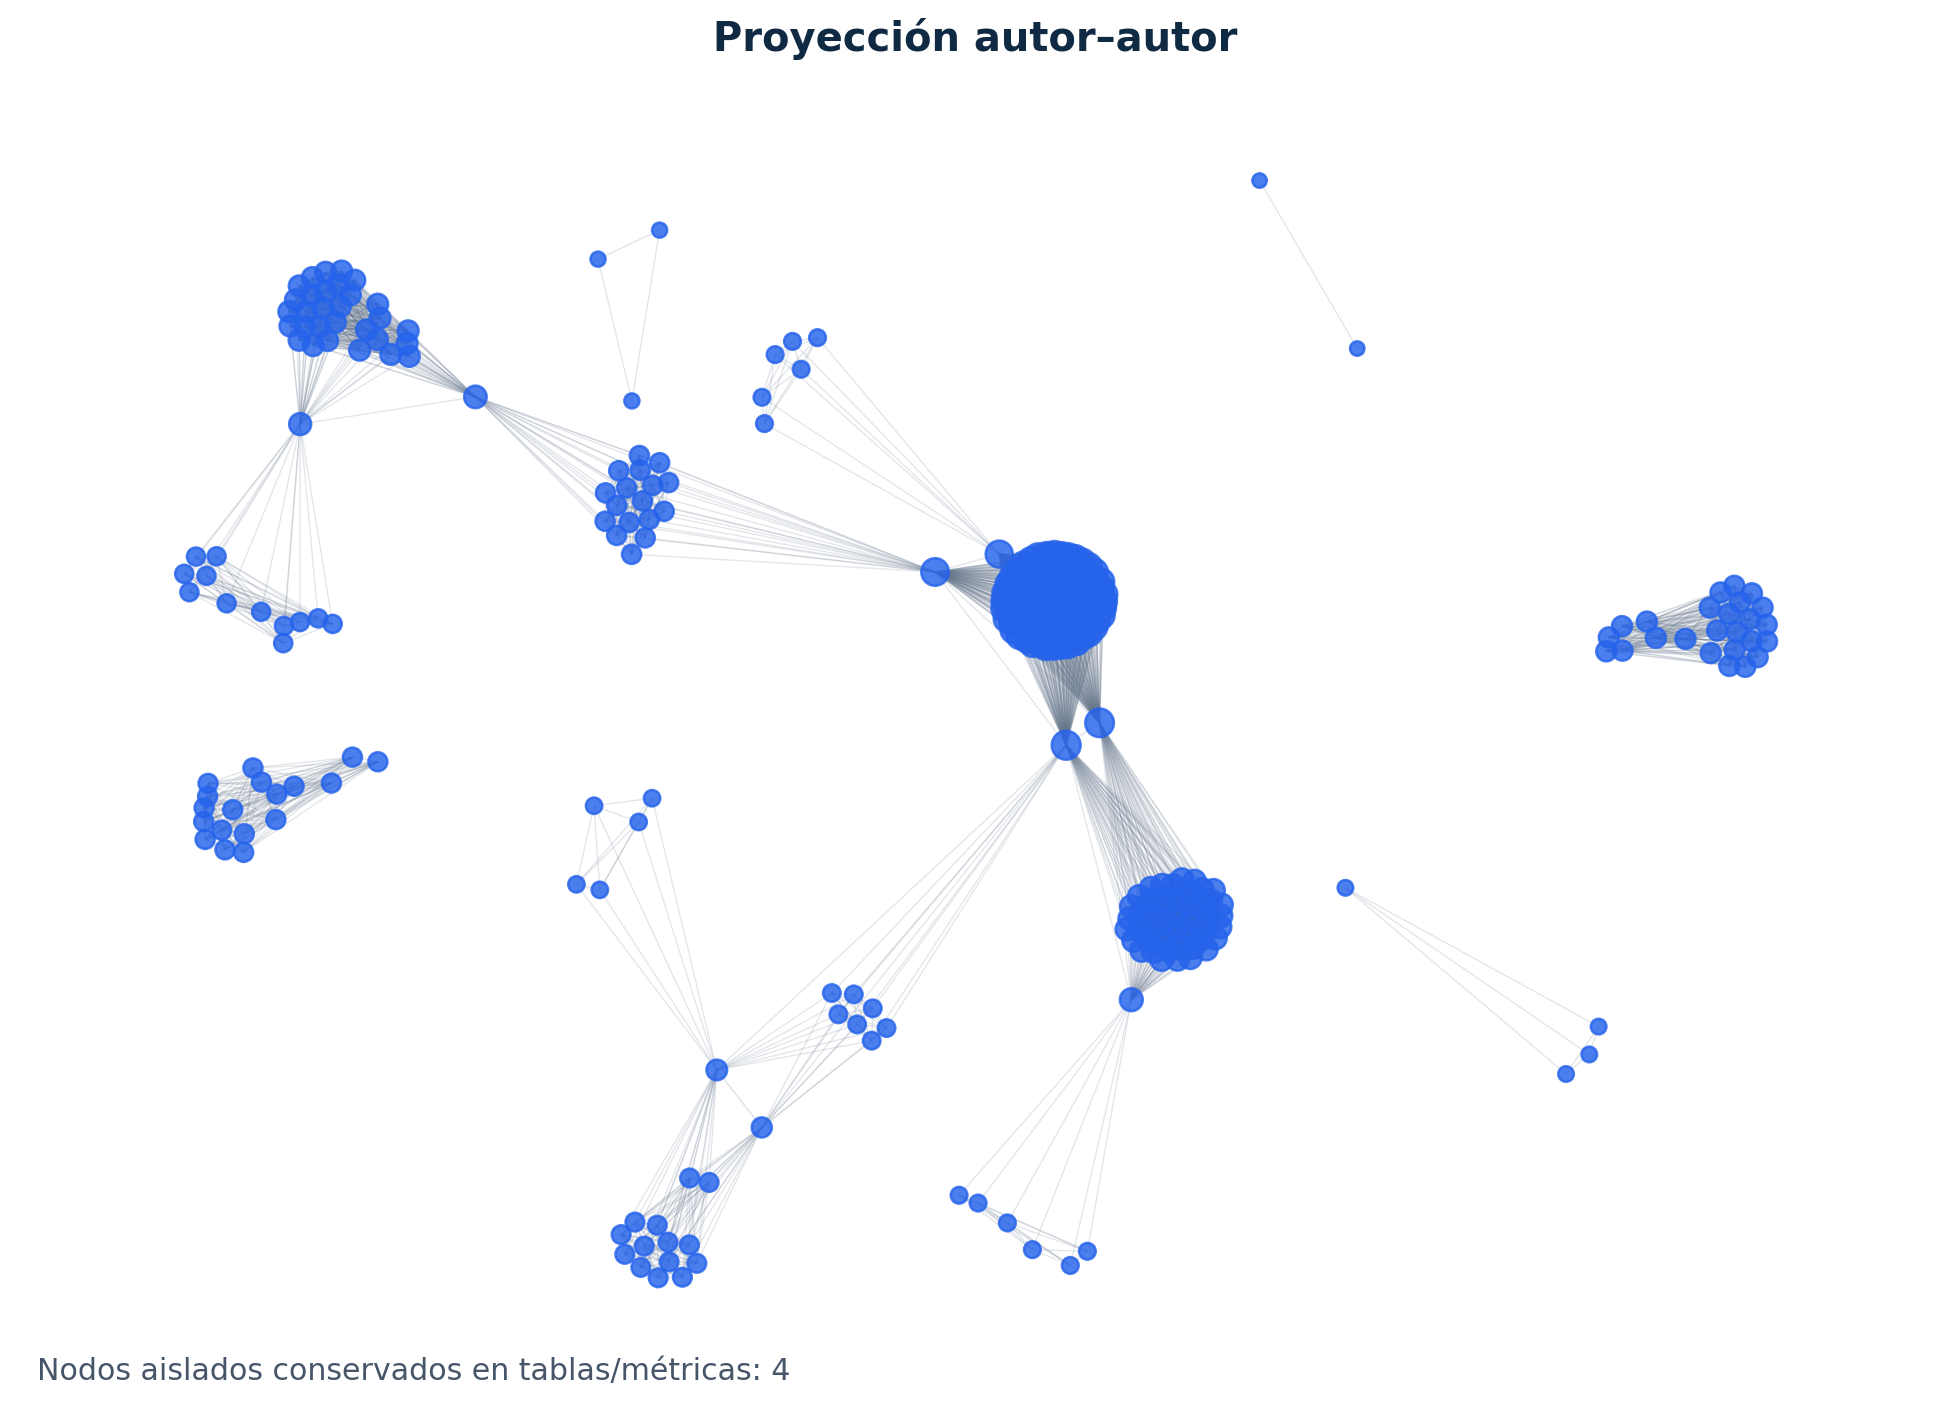
\includegraphics[width=0.82\textwidth]{proyeccion_autores.png}
\caption{Proyección autor--autor; el peso representa videos compartidos.}
\label{fig:autores}
\end{figure}

\begin{figure}[H]
\centering
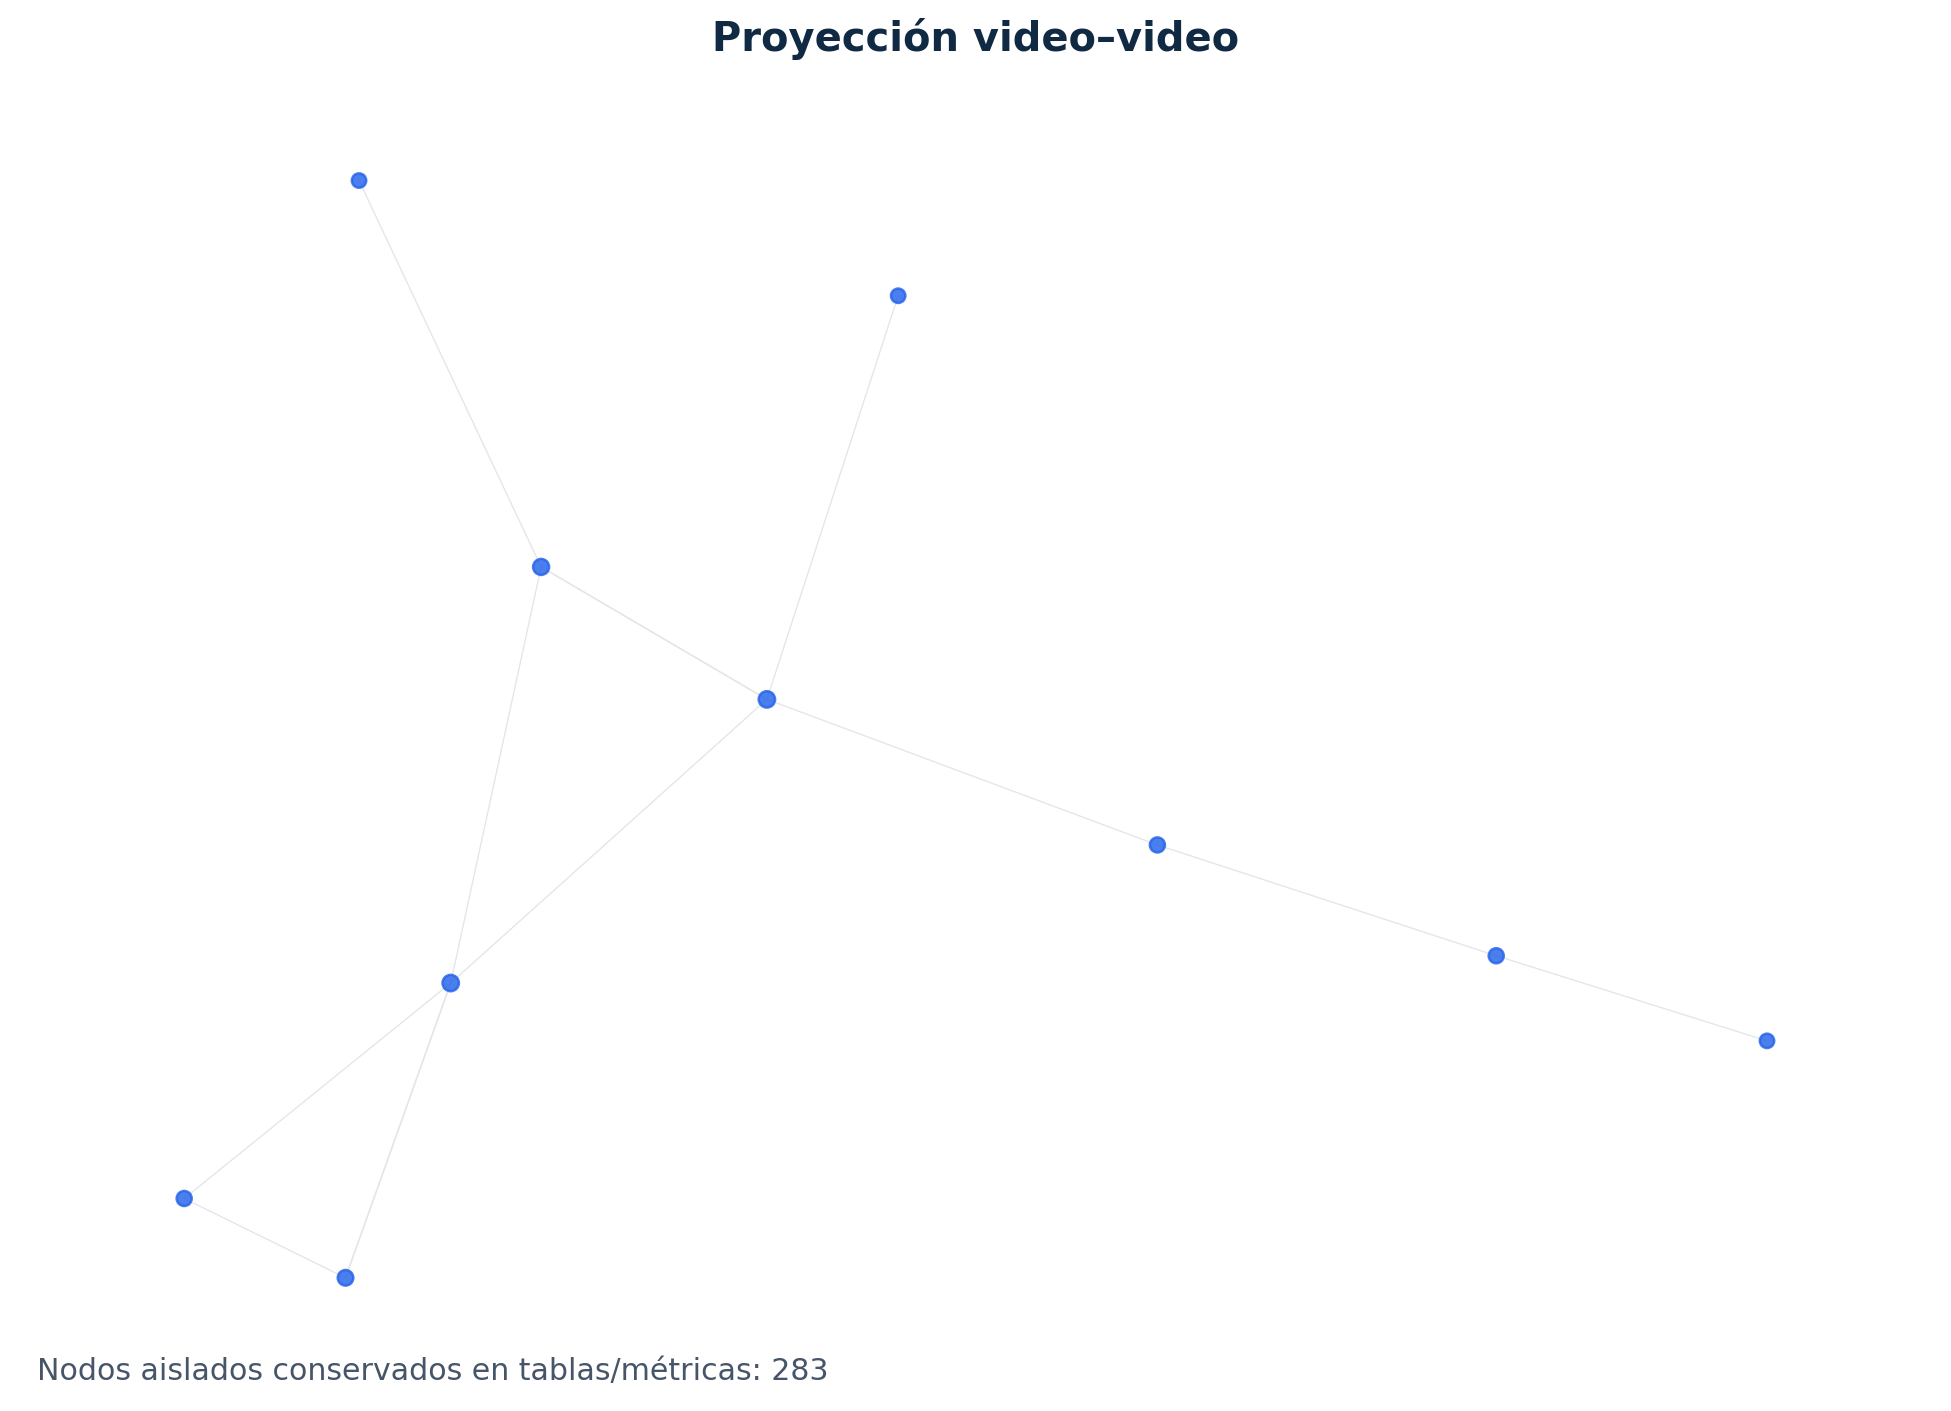
\includegraphics[width=0.82\textwidth]{proyeccion_videos.png}
\caption{Proyección video--video; el peso representa autores compartidos.}
\label{fig:videos}
\end{figure}

La proyección de autores conecta a dos cuentas cuando comentaron el mismo video; aproxima copresencia en espacios de participación, no interacción. La proyección de videos conecta contenidos que comparten al menos un autor y muestra solapamiento de audiencias. Los pesos cuentan videos o autores compartidos, respectivamente.

\section{Topología y fragmentación}

\begin{table}[H]
\centering
\caption{Métricas estructurales principales.}
\resizebox{\textwidth}{!}{%
\begin{tabular}{lrrrrrrrr}
\toprule
Red & Nodos & Aristas & Aislados & Densidad & Grado medio & Componentes & Mayor comp. & Transitividad\\
\midrule
Bipartita & 625 & 343 & 274 & 0.00176 & 1.10 & 284 & 286 & 0.000\\
Autores & 332 & 10,732 & 4 & 0.19532 & 64.65 & 10 & 276 & 0.984\\
Videos & 293 & 11 & 283 & 0.00026 & 0.08 & 284 & 10 & 0.316\\
\bottomrule
\end{tabular}}
\end{table}

\begin{figure}[H]
\centering
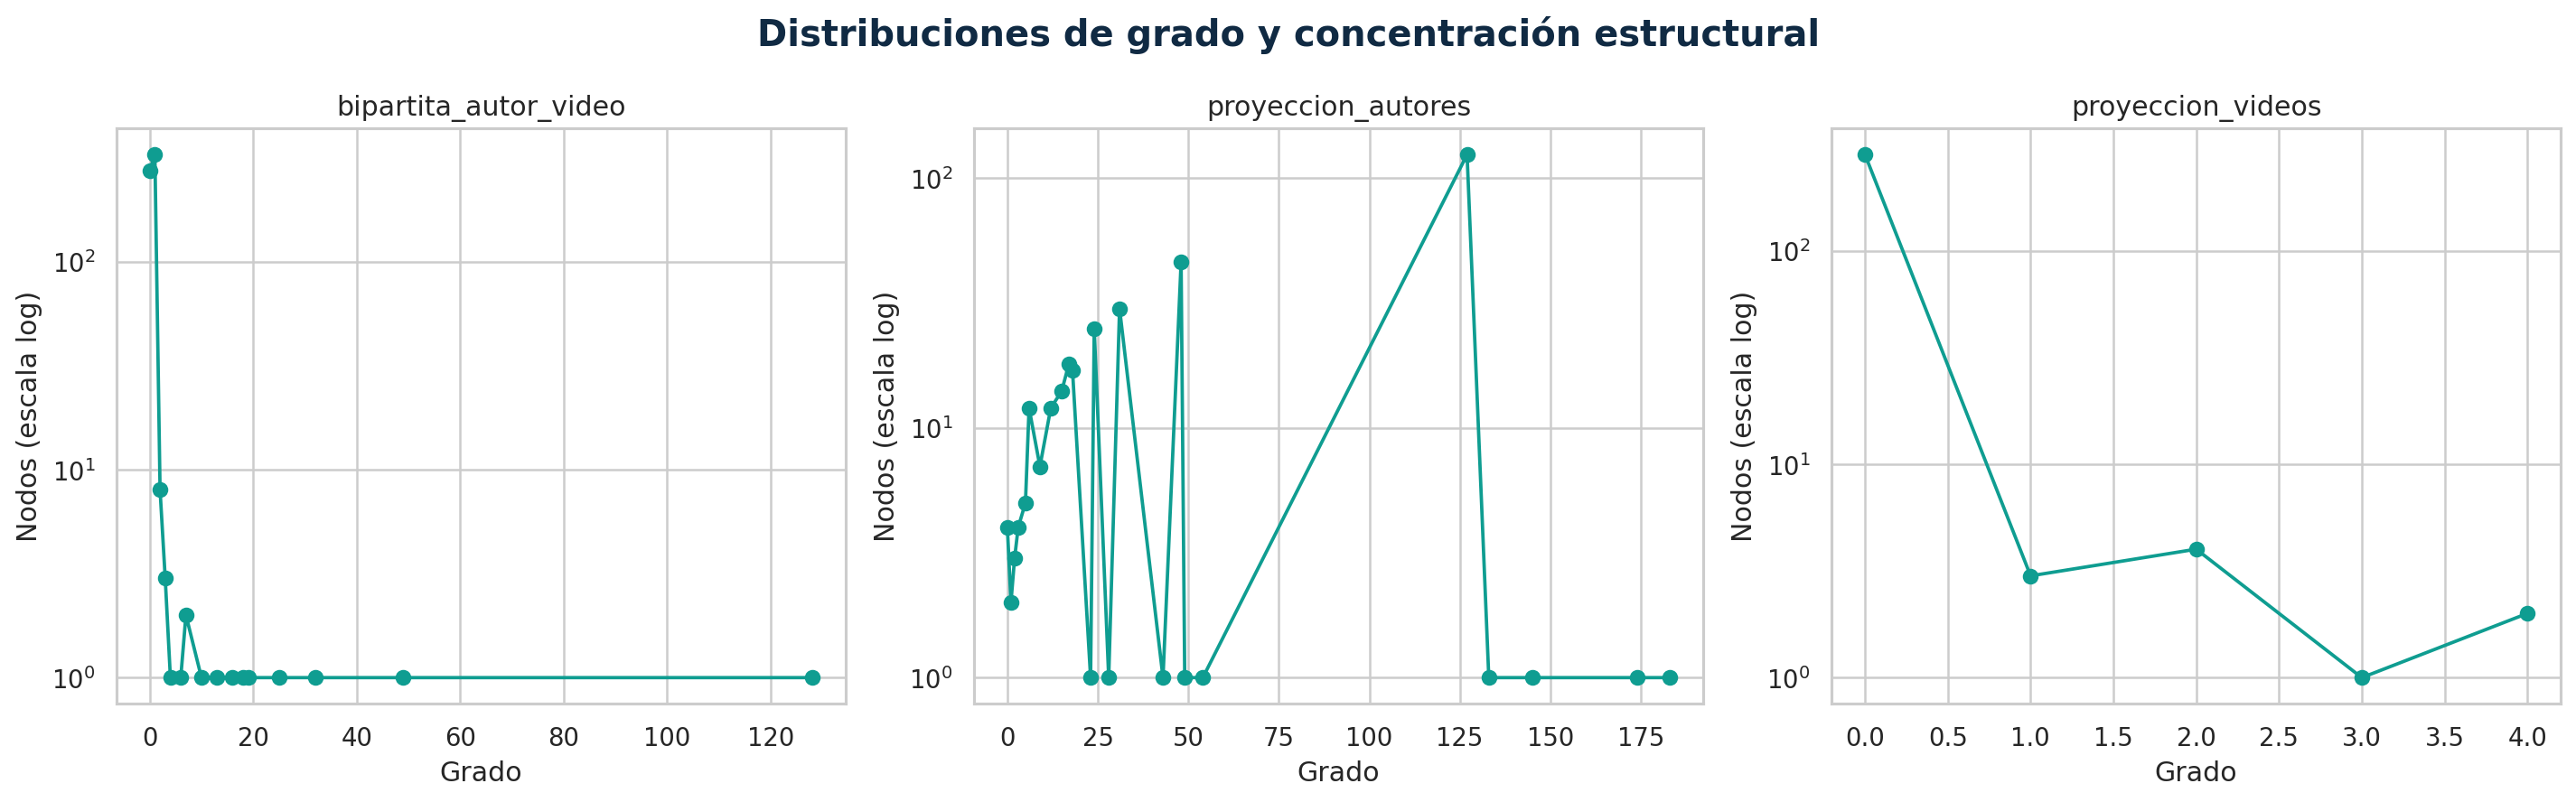
\includegraphics[width=0.98\textwidth]{distribuciones_grado.png}
\caption{Distribuciones de grado de las tres redes.}
\label{fig:grado}
\end{figure}

La red bipartita es dispersa y fragmentada por la falta de comentarios para la mayoría de videos. Su transitividad es cero por construcción: un grafo estrictamente bipartito no contiene triángulos. La proyección de autores es mucho más densa y alcanza transitividad 0.984, pero esta cifra está inflada estructuralmente porque todos los autores de un mismo video forman un clique. No representa cohesión interpersonal comprobada. La proyección de videos confirma un solapamiento muy limitado: solo diez videos tienen al menos una conexión.

La cohesión se midió en la componente conexa mayor mediante conectividad de nodos y de aristas. La conectividad de nodos es 1 en las tres redes: existe al menos un punto cuya remoción puede separar la componente. La conectividad de aristas es 1 en la bipartita y la proyección de videos, y 5 en la proyección de autores. Los diámetros de las componentes mayores también se conservan en \texttt{metricas\_redes.csv}.

Los aislados son aislamiento \emph{observado}; no prueban desinterés o inexistencia de audiencia. Pueden reflejar que no se descargaron comentarios, que la API devolvió cobertura parcial o que el procedimiento de búsqueda no capturó actividad.

\section{Comunidades}

Se eligió la proyección autor--autor porque permite estudiar conjuntos de usuarios que concurren en videos semejantes. Se aplicó Louvain ponderado con semilla 42, donde el peso es el número de videos compartidos. Los cuatro aislados de la proyección se conservaron en las métricas pero se excluyeron de la optimización de modularidad porque no aportan enlaces.

\begin{figure}[H]
\centering
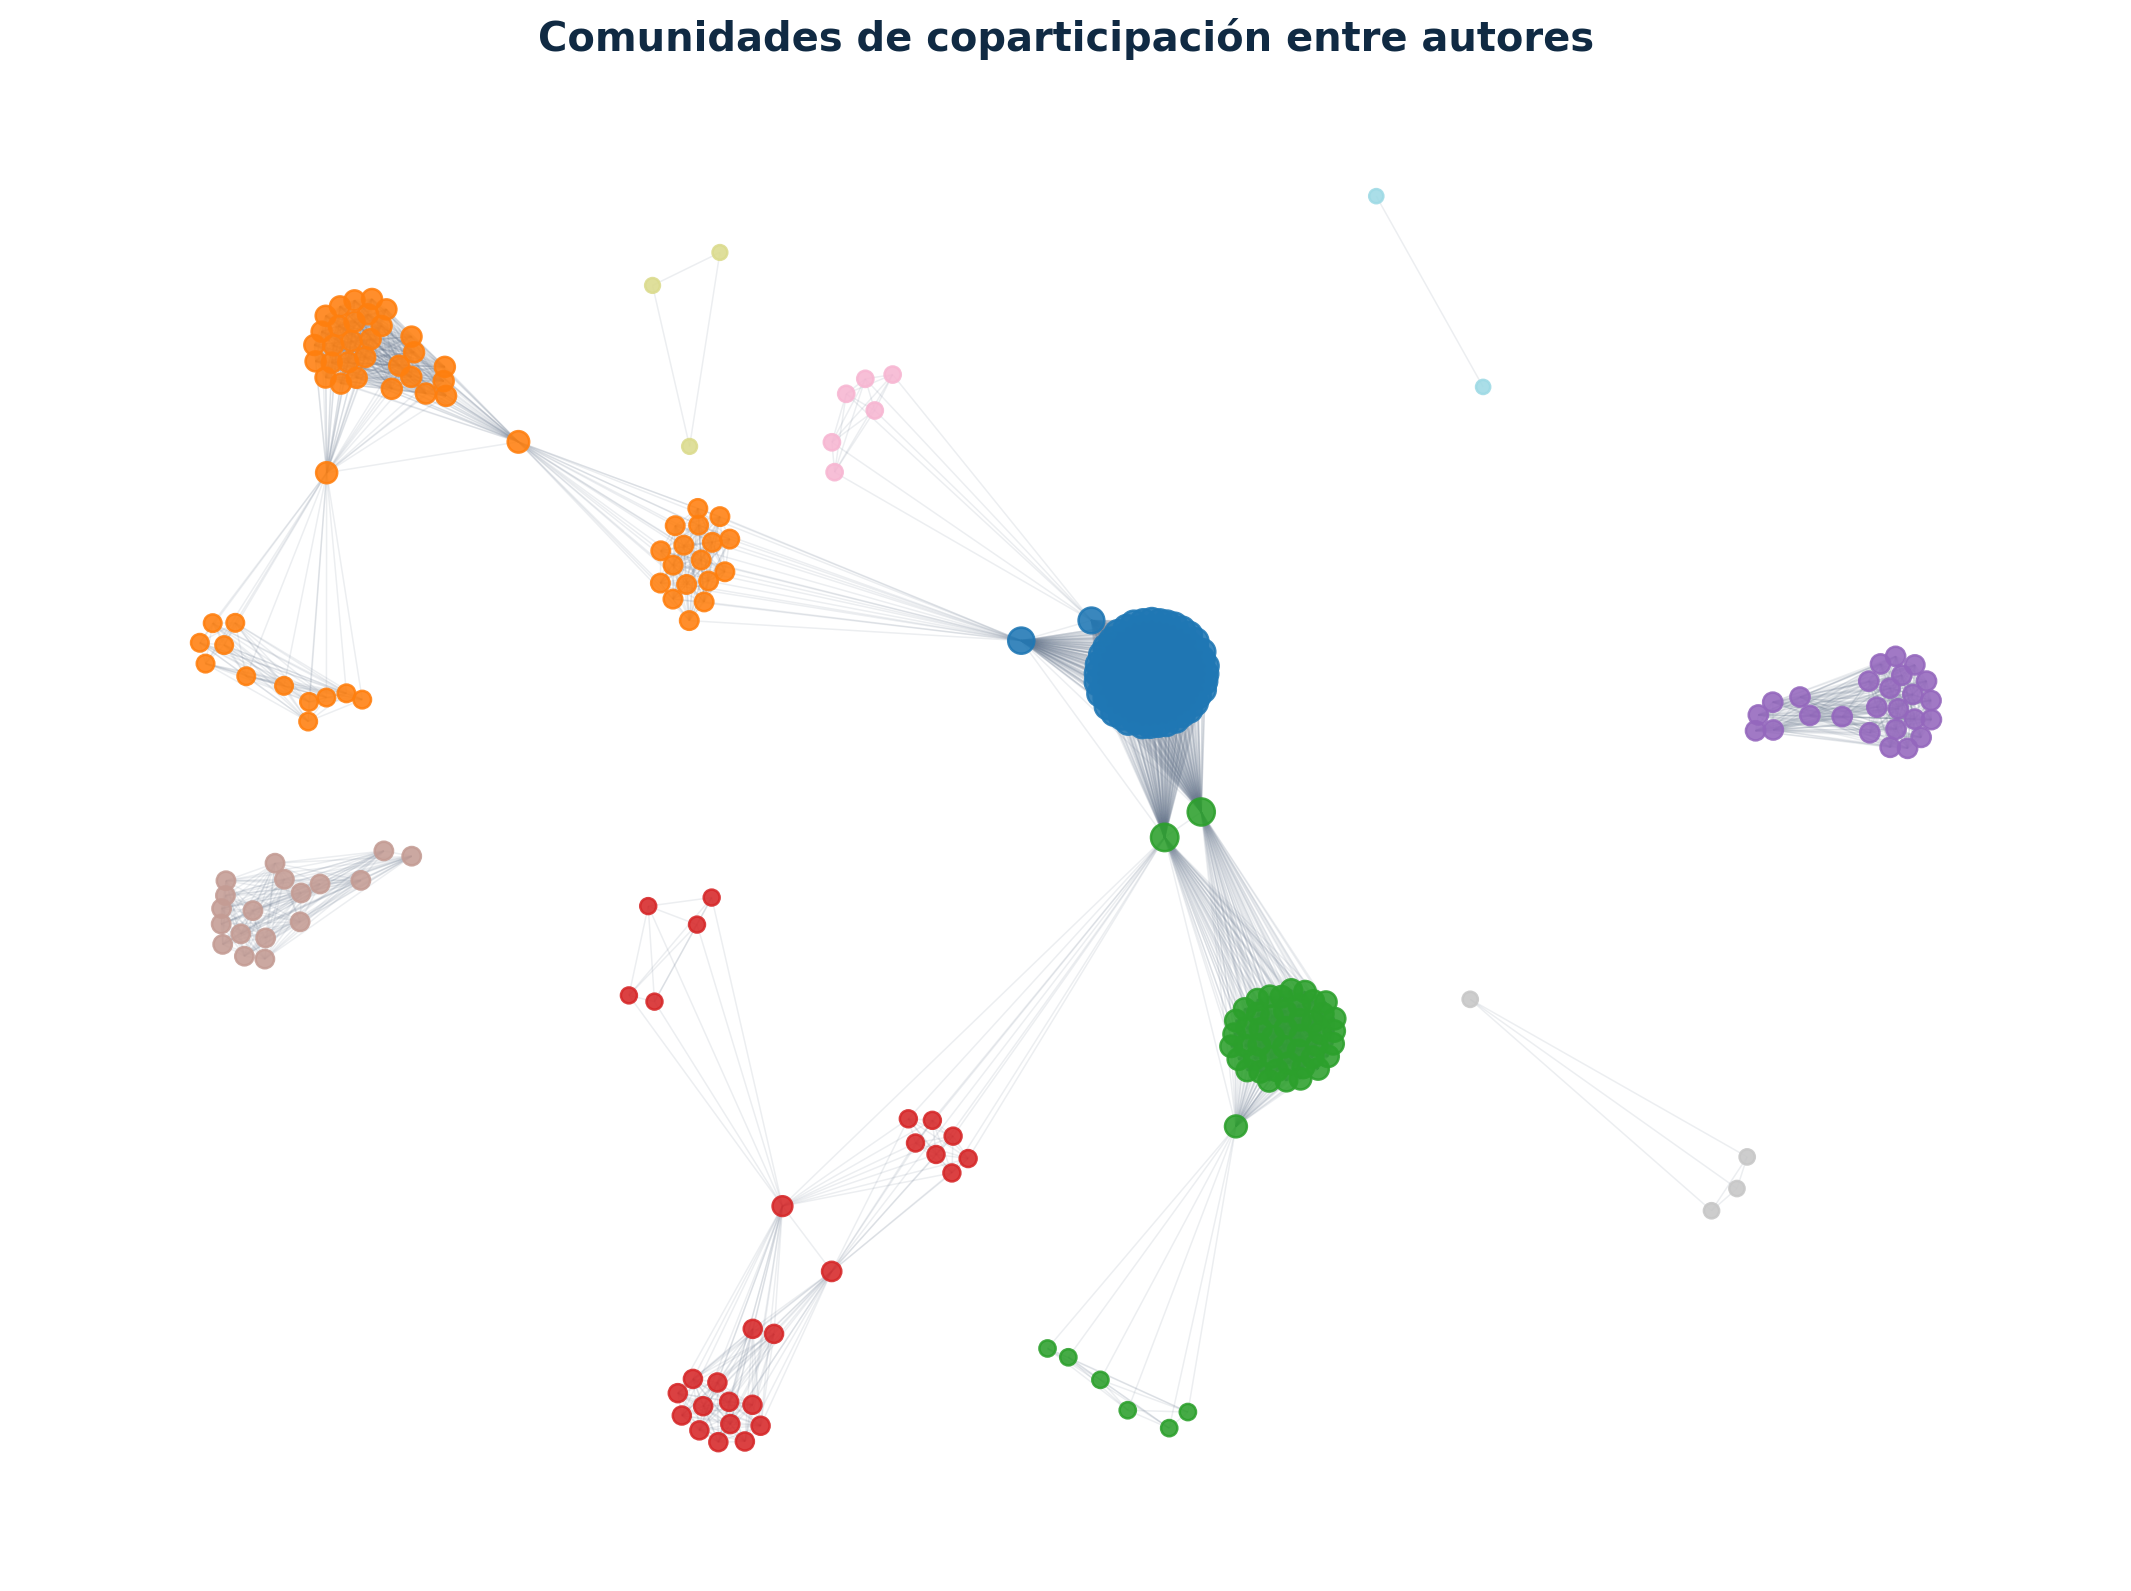
\includegraphics[width=0.88\textwidth]{comunidades_autores.png}
\caption{Diez comunidades de coparticipación detectadas mediante Louvain.}
\label{fig:comunidades}
\end{figure}

La modularidad fue 0.395. La comunidad 1 reúne 126 autores y 161 comentarios, con vocabulario sobre pueblo, dinero y diputados; RoBERTuito clasificó 80.7\% de sus comentarios como negativos. La comunidad 2 contiene 61 autores y 83 comentarios relacionados con presidencia, Guatemala y gobierno: 44.6\% fueron negativos, 27.7\% neutrales y 27.7\% positivos. La comunidad 3 contiene 55 autores y 60 comentarios, destacando USAC, universidad y corrupción: 61.7\% fueron negativos, 18.3\% neutrales y 20.0\% positivos. Estas comunidades reflejan agrupación por contenidos compartidos; no son grupos sociales confirmados. El detalle de sentimiento por comunidad está en \texttt{sentimiento\_por\_comunidad.csv} y se explica en la Sección~\ref{sec:sentimiento}.

\section{Nodos centrales y participantes puente}

Se calcularon grado, grado ponderado, intermediación (sobre distancia $=1/\text{peso}$), centralidad armónica y PageRank ponderado para autores y videos (\texttt{centralidad\_autores.csv}, \texttt{centralidad\_videos.csv}). Se usó centralidad armónica en lugar de cercanía clásica porque la red está fragmentada (10 componentes de autores, 284 de videos) y la cercanía clásica no está definida entre componentes distintos; PageRank ponderado complementa el grado descontando la centralidad heredada de vecinos muy conectados. Se descartó la centralidad de vectores propios porque, con tantos componentes, se concentra en la componente dominante y asigna cero al resto.

\begin{figure}[H]
\centering
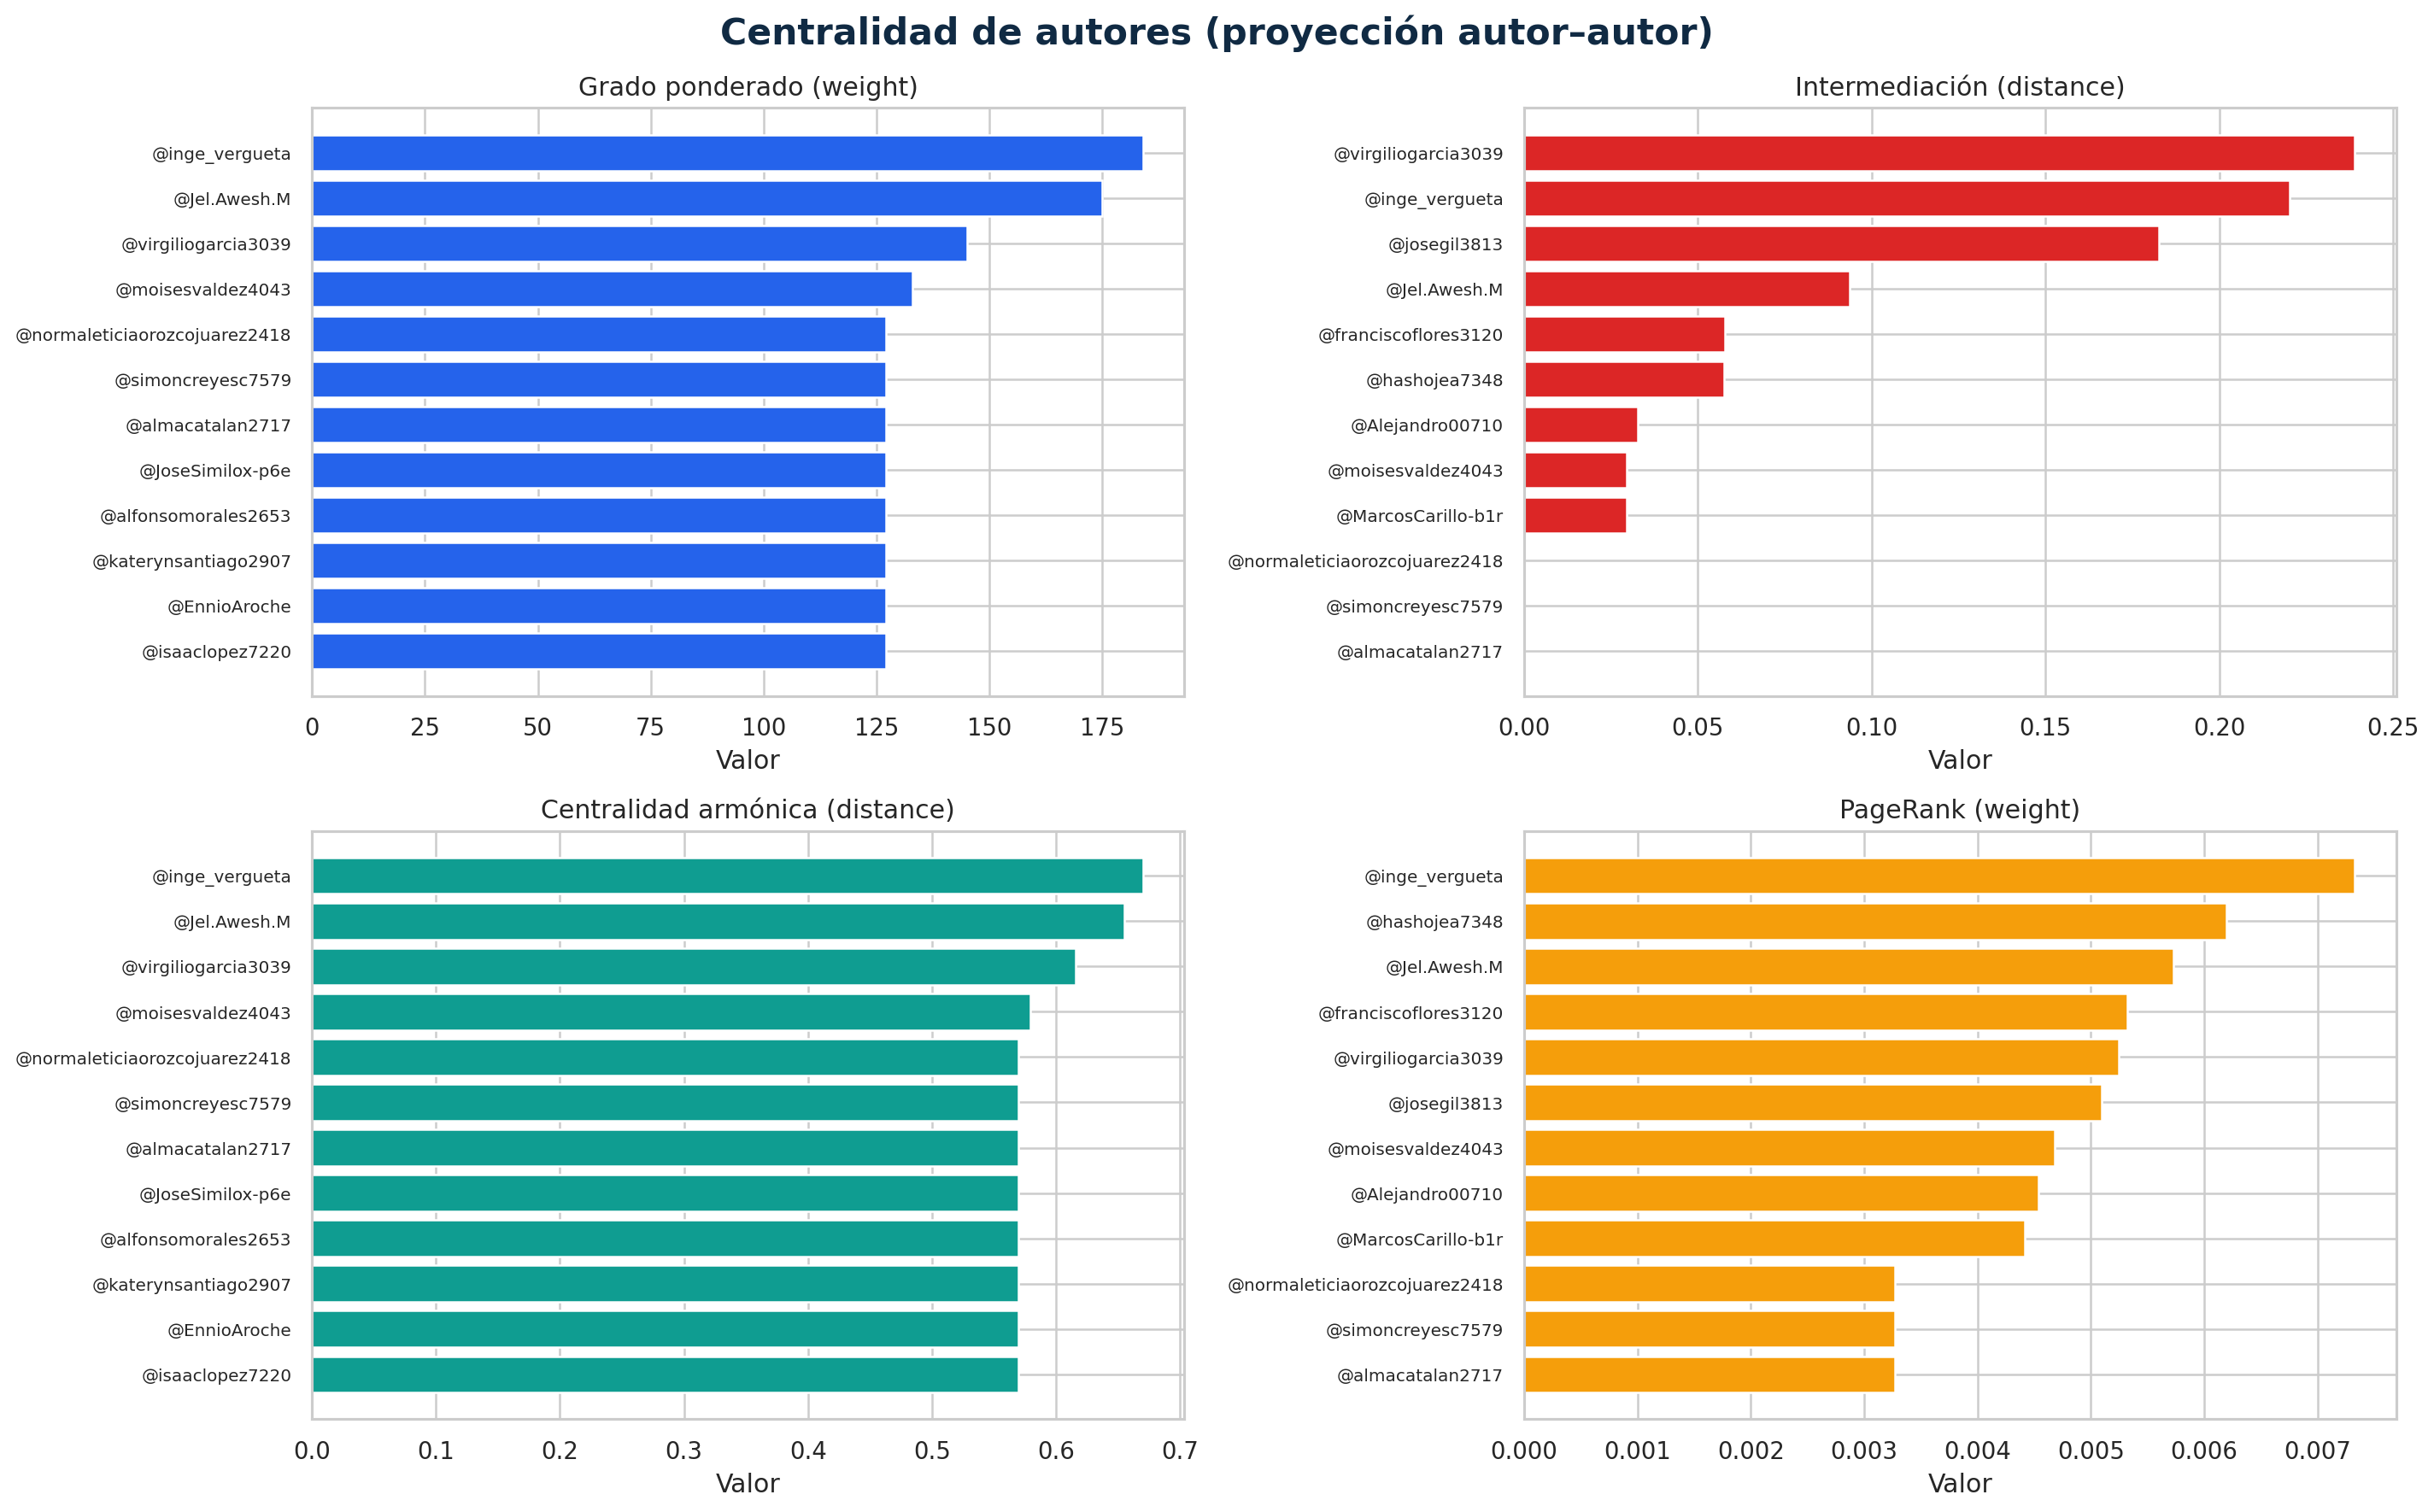
\includegraphics[width=0.9\textwidth]{centralidad_autores.png}
\caption{Centralidad de autores (proyección autor--autor).}
\end{figure}

\begin{figure}[H]
\centering
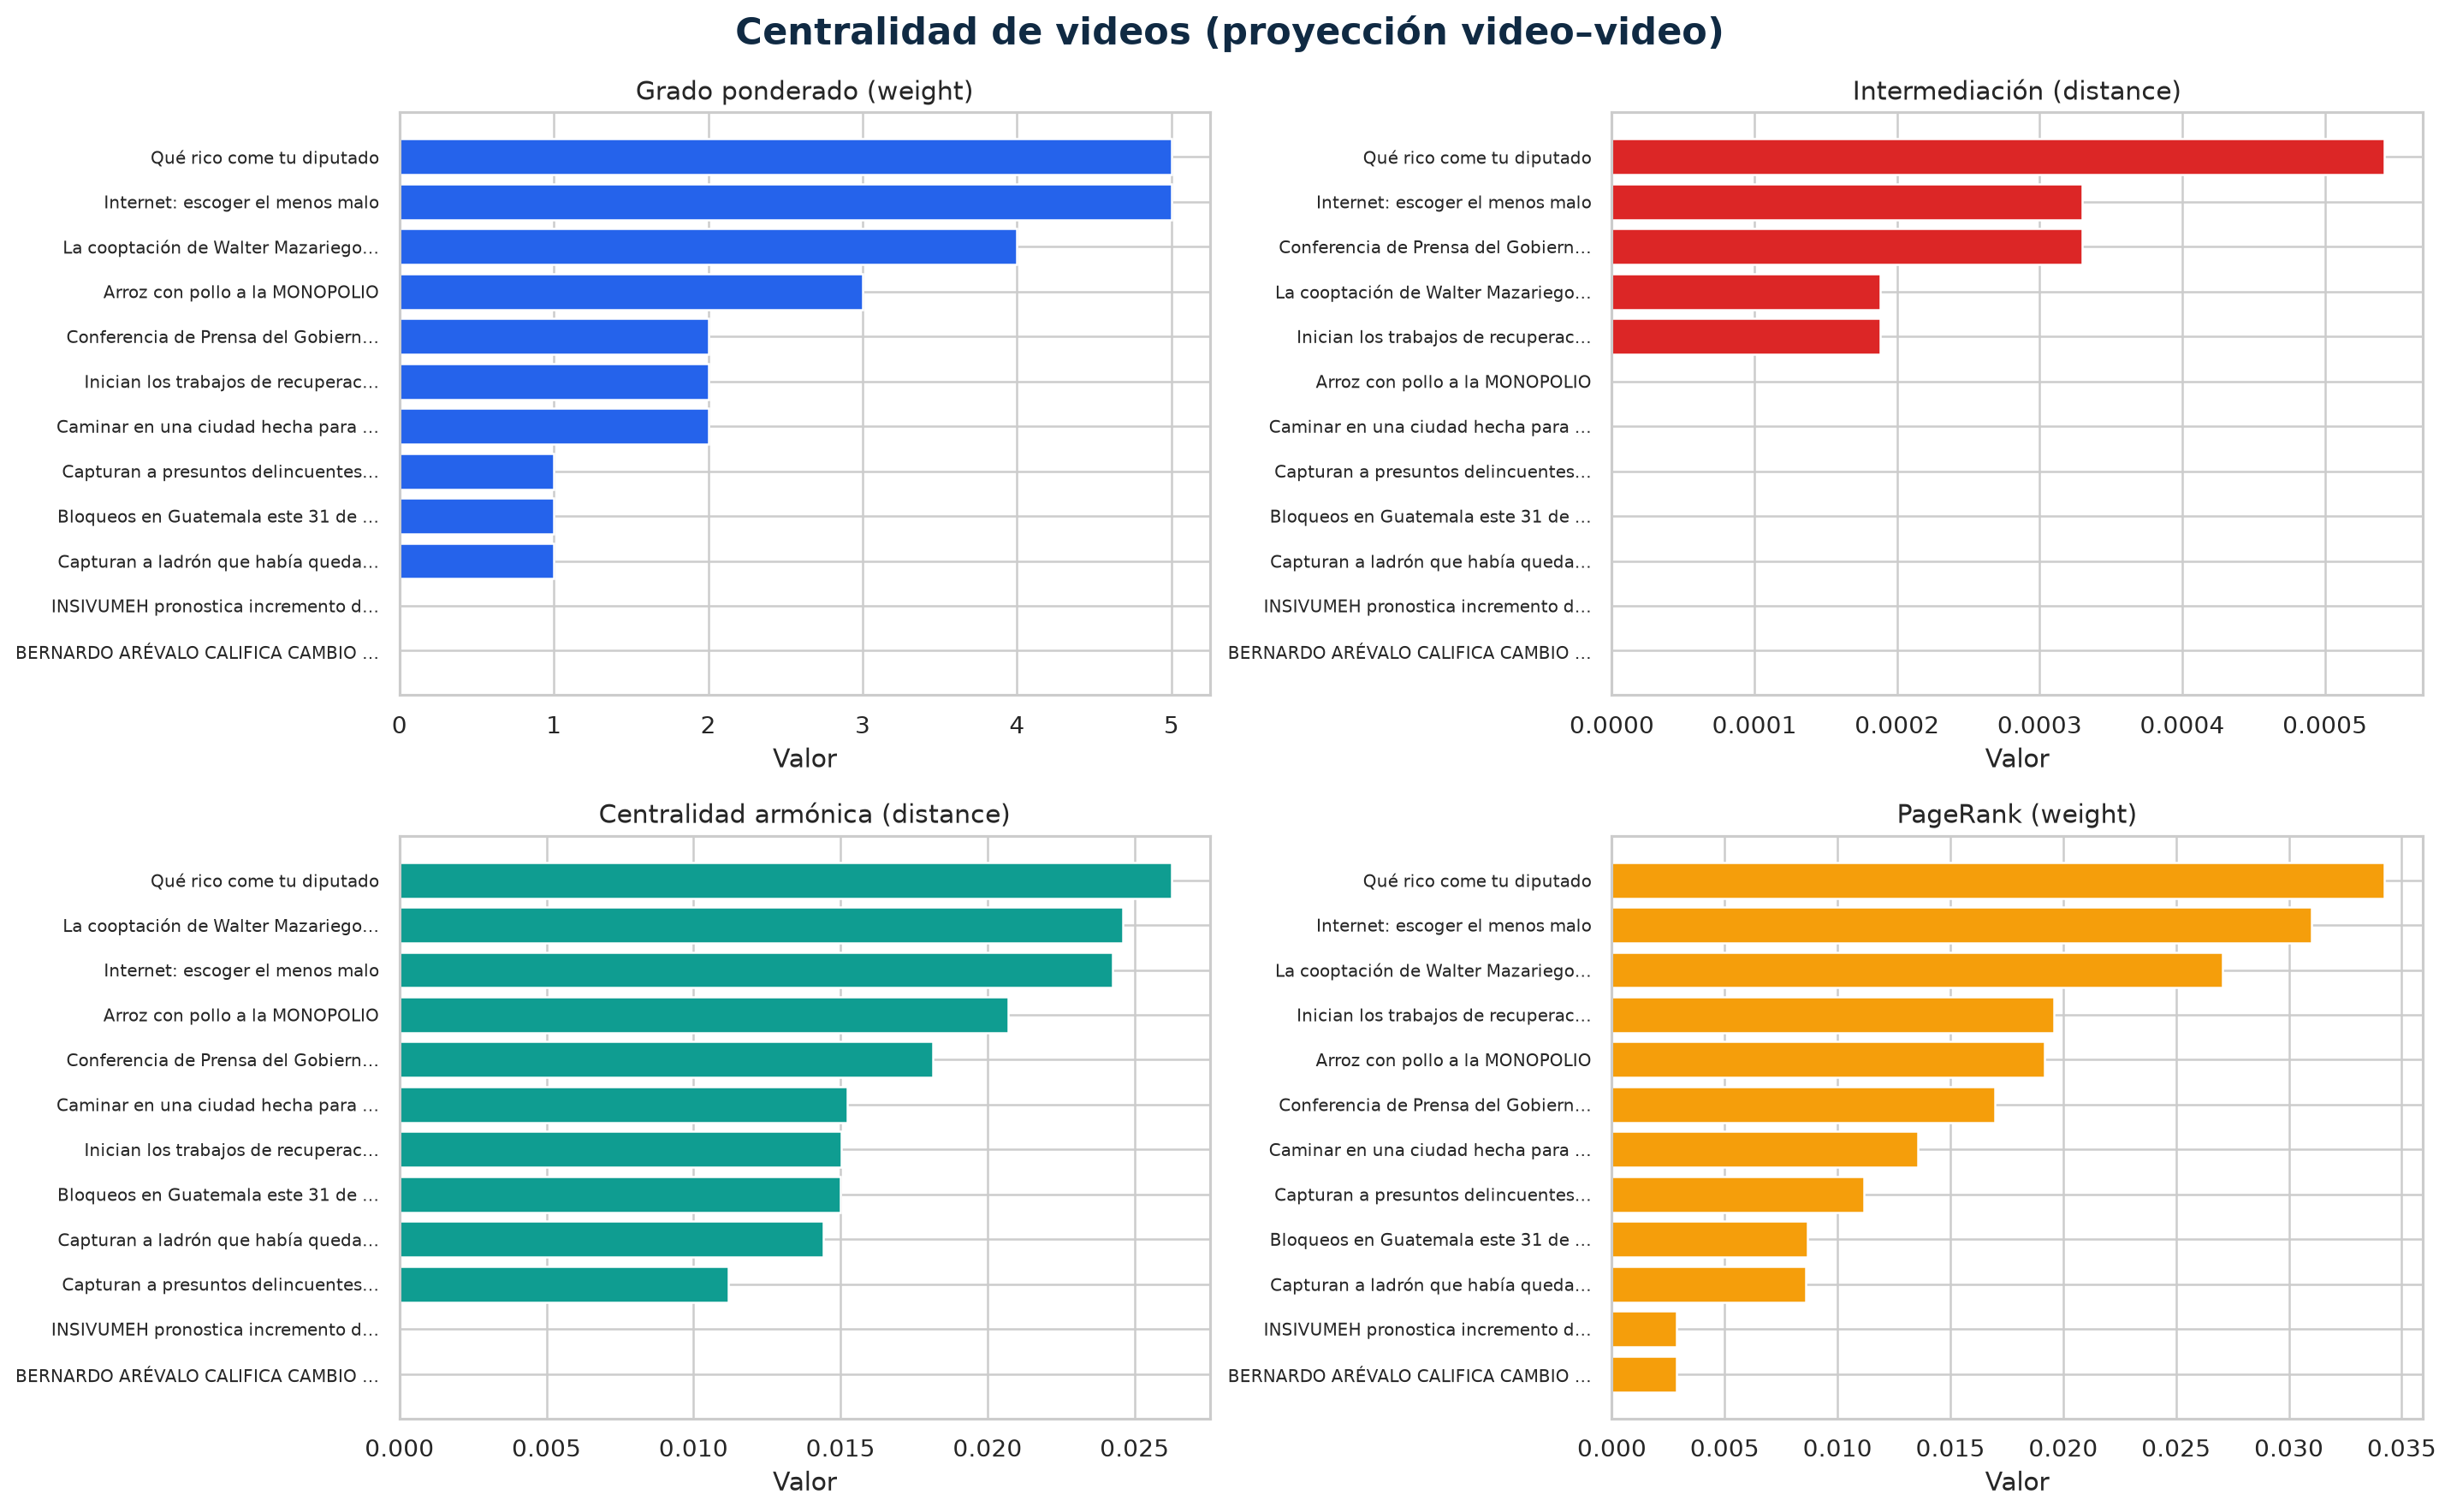
\includegraphics[width=0.9\textwidth]{centralidad_videos.png}
\caption{Centralidad de videos (proyección video--video).}
\end{figure}

Solo 9 de 332 autores (2.7\%) comentaron en más de un video; únicamente esos 9 tienen intermediación positiva, 7 son puntos de articulación y 4 quedan aislados por ser el único comentarista de su video. Los tres primeros por intermediación son @virgiliogarcia3039 (2 videos, intermediación 0.239), @inge\_vergueta (3 videos, 0.220) y @josegil3813 (2 videos, 0.183). En videos, 10 de 293 comparten autores; 5 son articuladores, y \emph{Qué rico come tu diputado} es el único cuya remoción parte la componente en tres.

\begin{figure}[H]
\centering
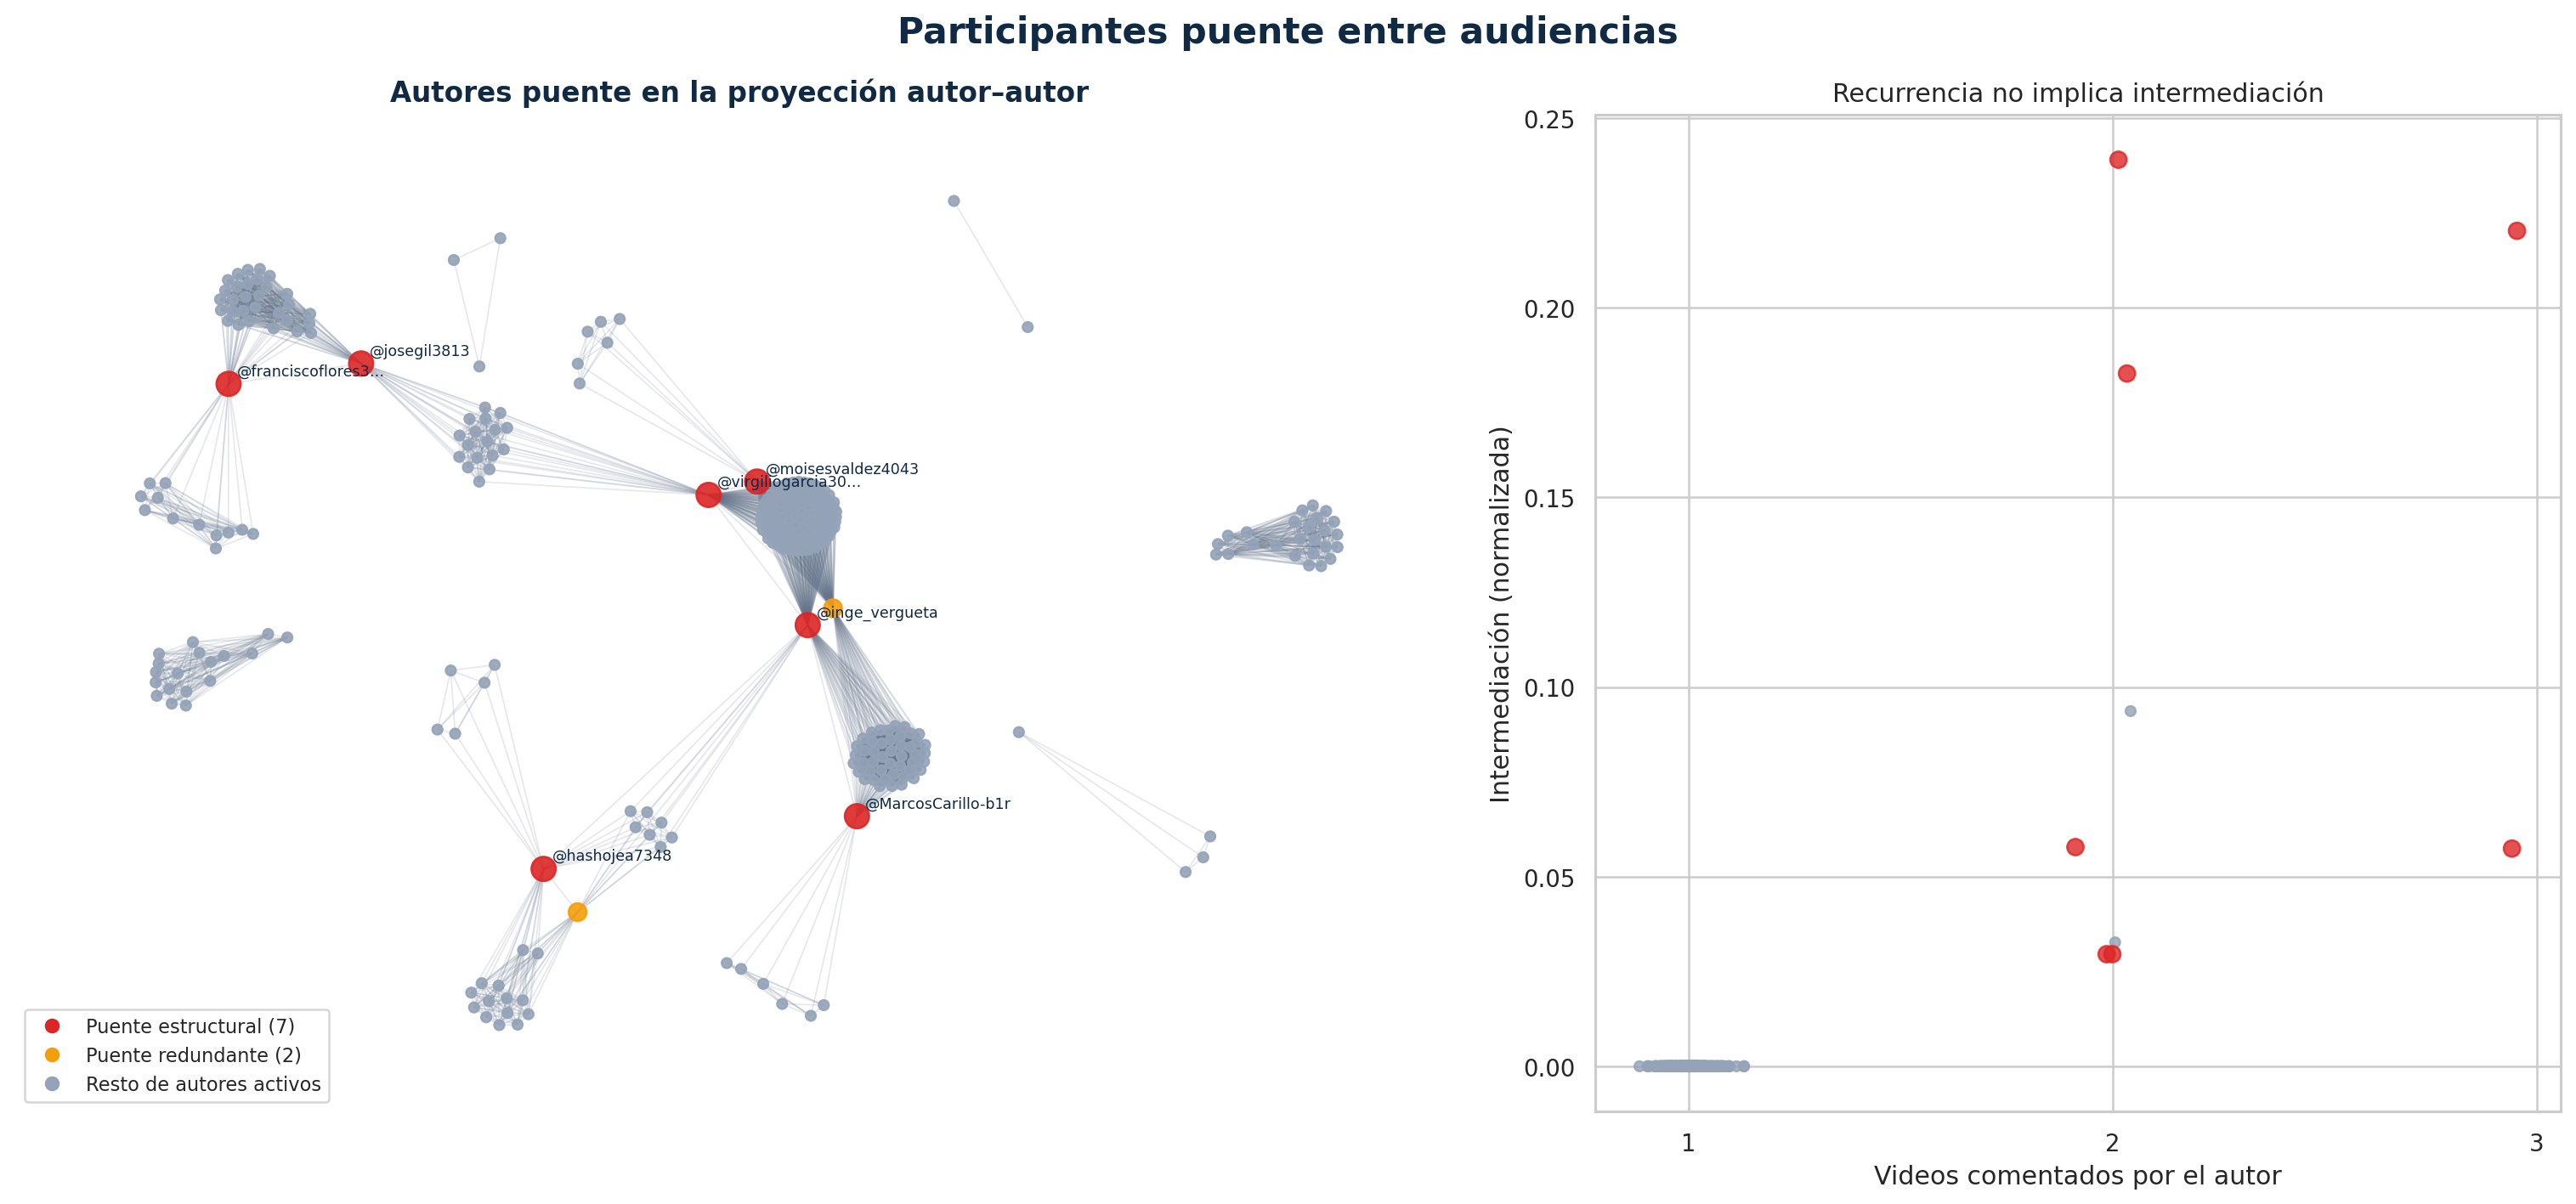
\includegraphics[width=0.9\textwidth]{autores_puente.png}
\caption{Autores puente identificados por intermediación y articulación.}
\end{figure}

\begin{figure}[H]
\centering
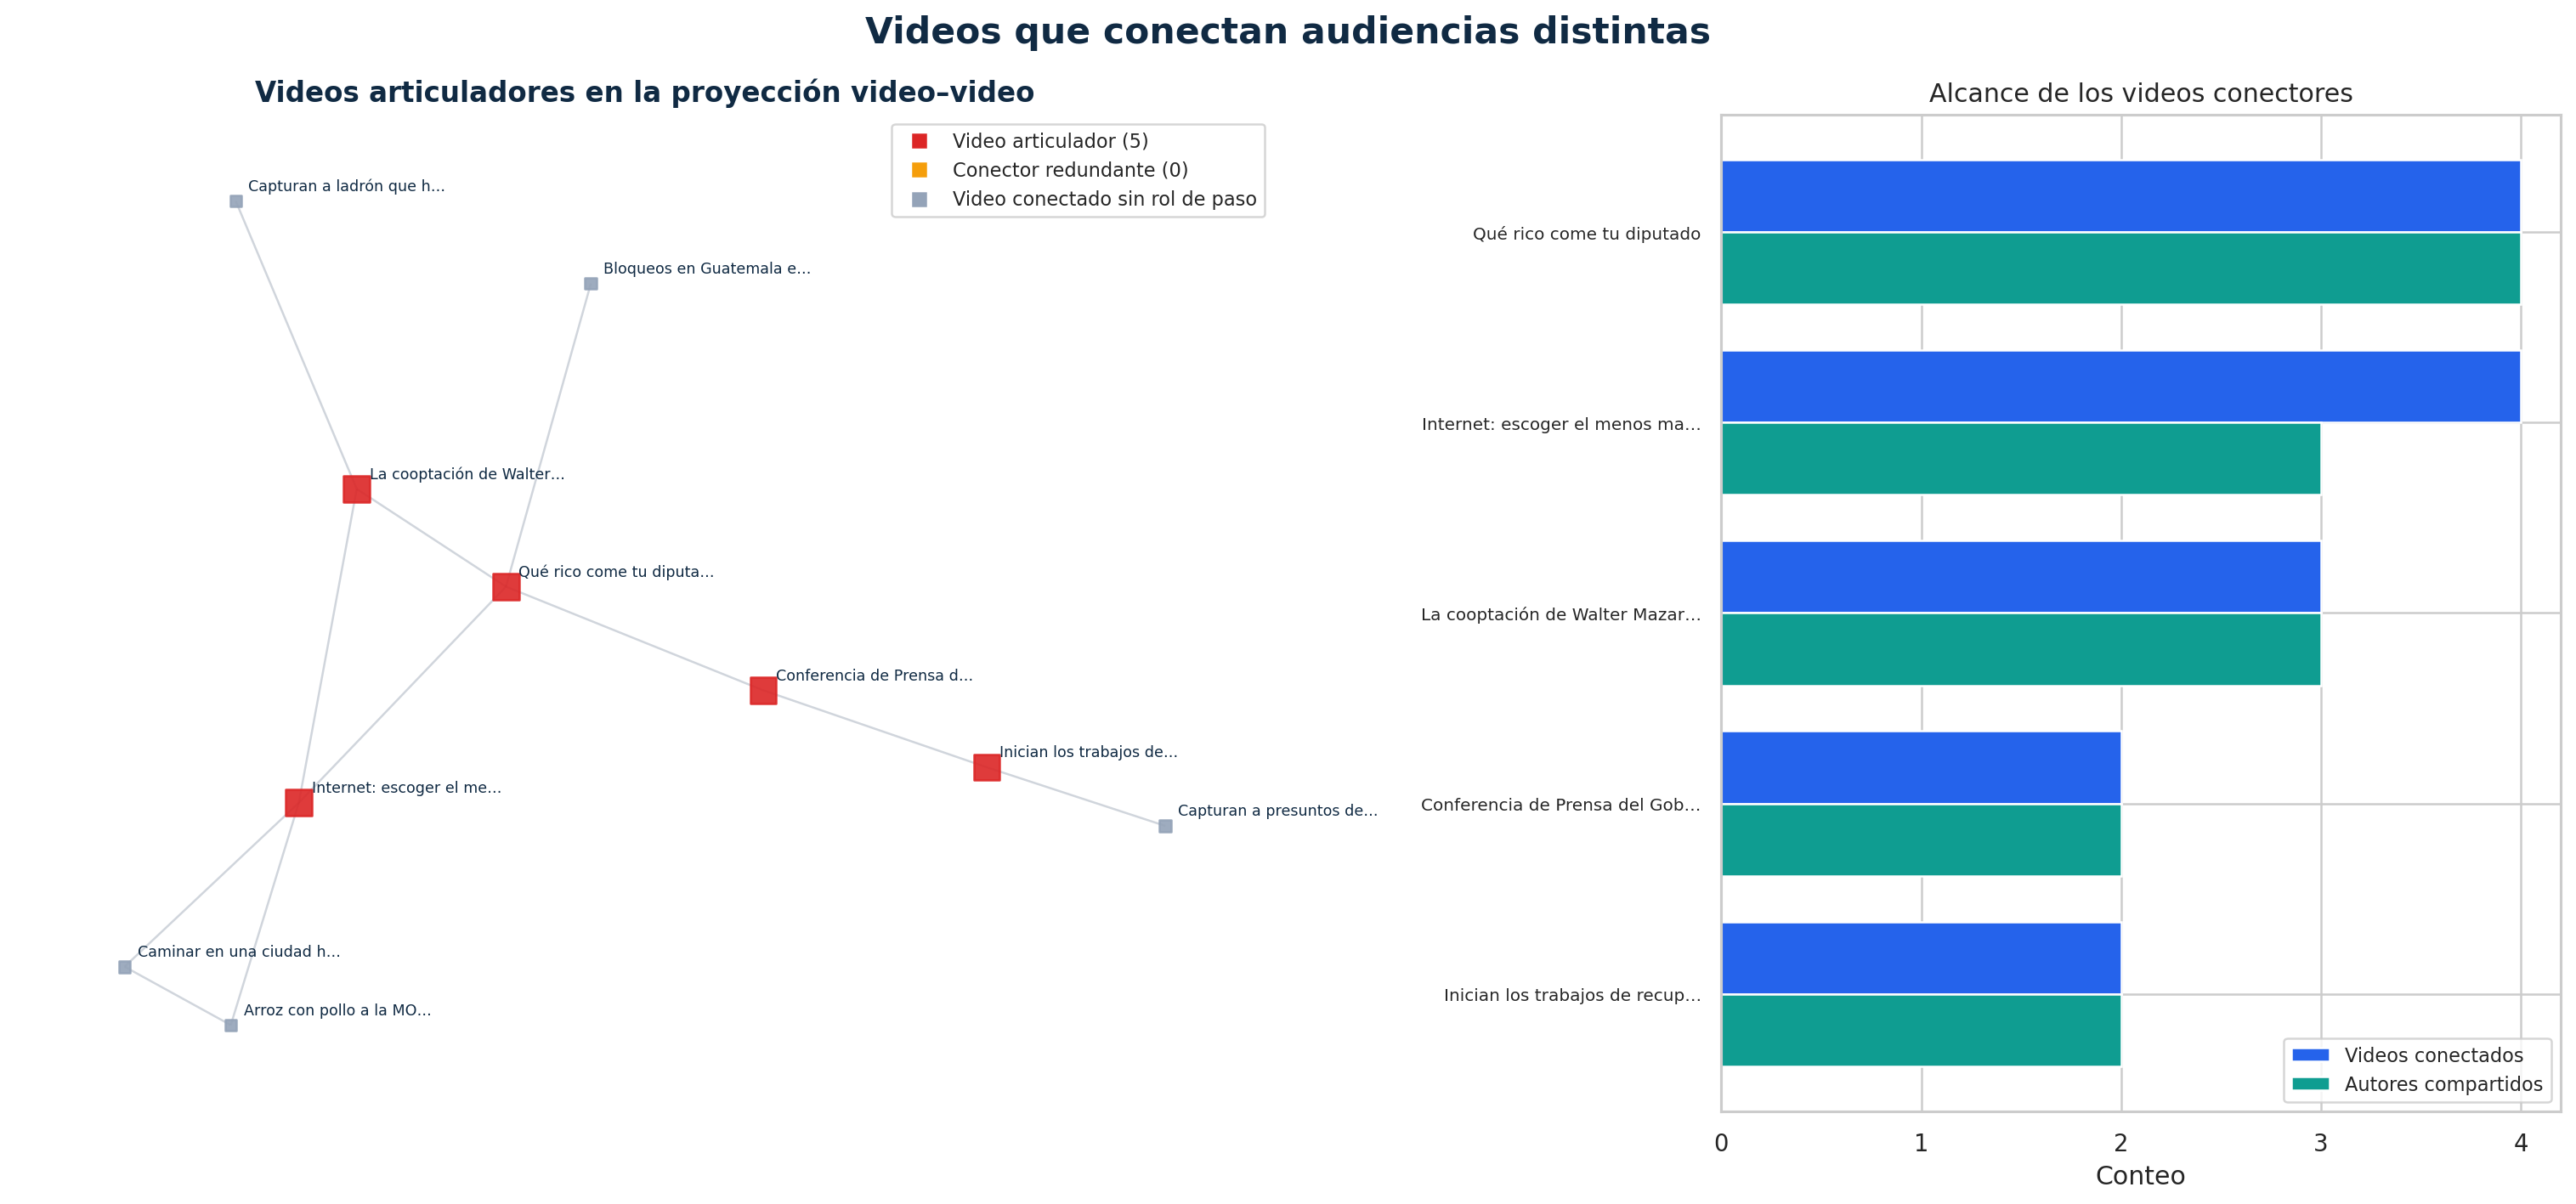
\includegraphics[width=0.9\textwidth]{videos_articuladores.png}
\caption{Videos articuladores de la proyección video--video.}
\end{figure}

Recurrencia (comentar en más de un video) es condición necesaria pero no suficiente para tener alta intermediación: entre los 9 autores recurrentes, la correlación de Spearman con intermediación cae a 0.208; lo decisivo es \emph{qué} videos conecta cada autor, no cuántos. Se evaluó la remoción de 25 nodos candidatos (\texttt{impacto\_remocion.csv}); 12 fragmentan la red. El caso extremo es @virgiliogarcia3039: al removerlo la componente mayor de autores cae de 276 a 214 nodos ($-22.5\%$).

\begin{figure}[H]
\centering
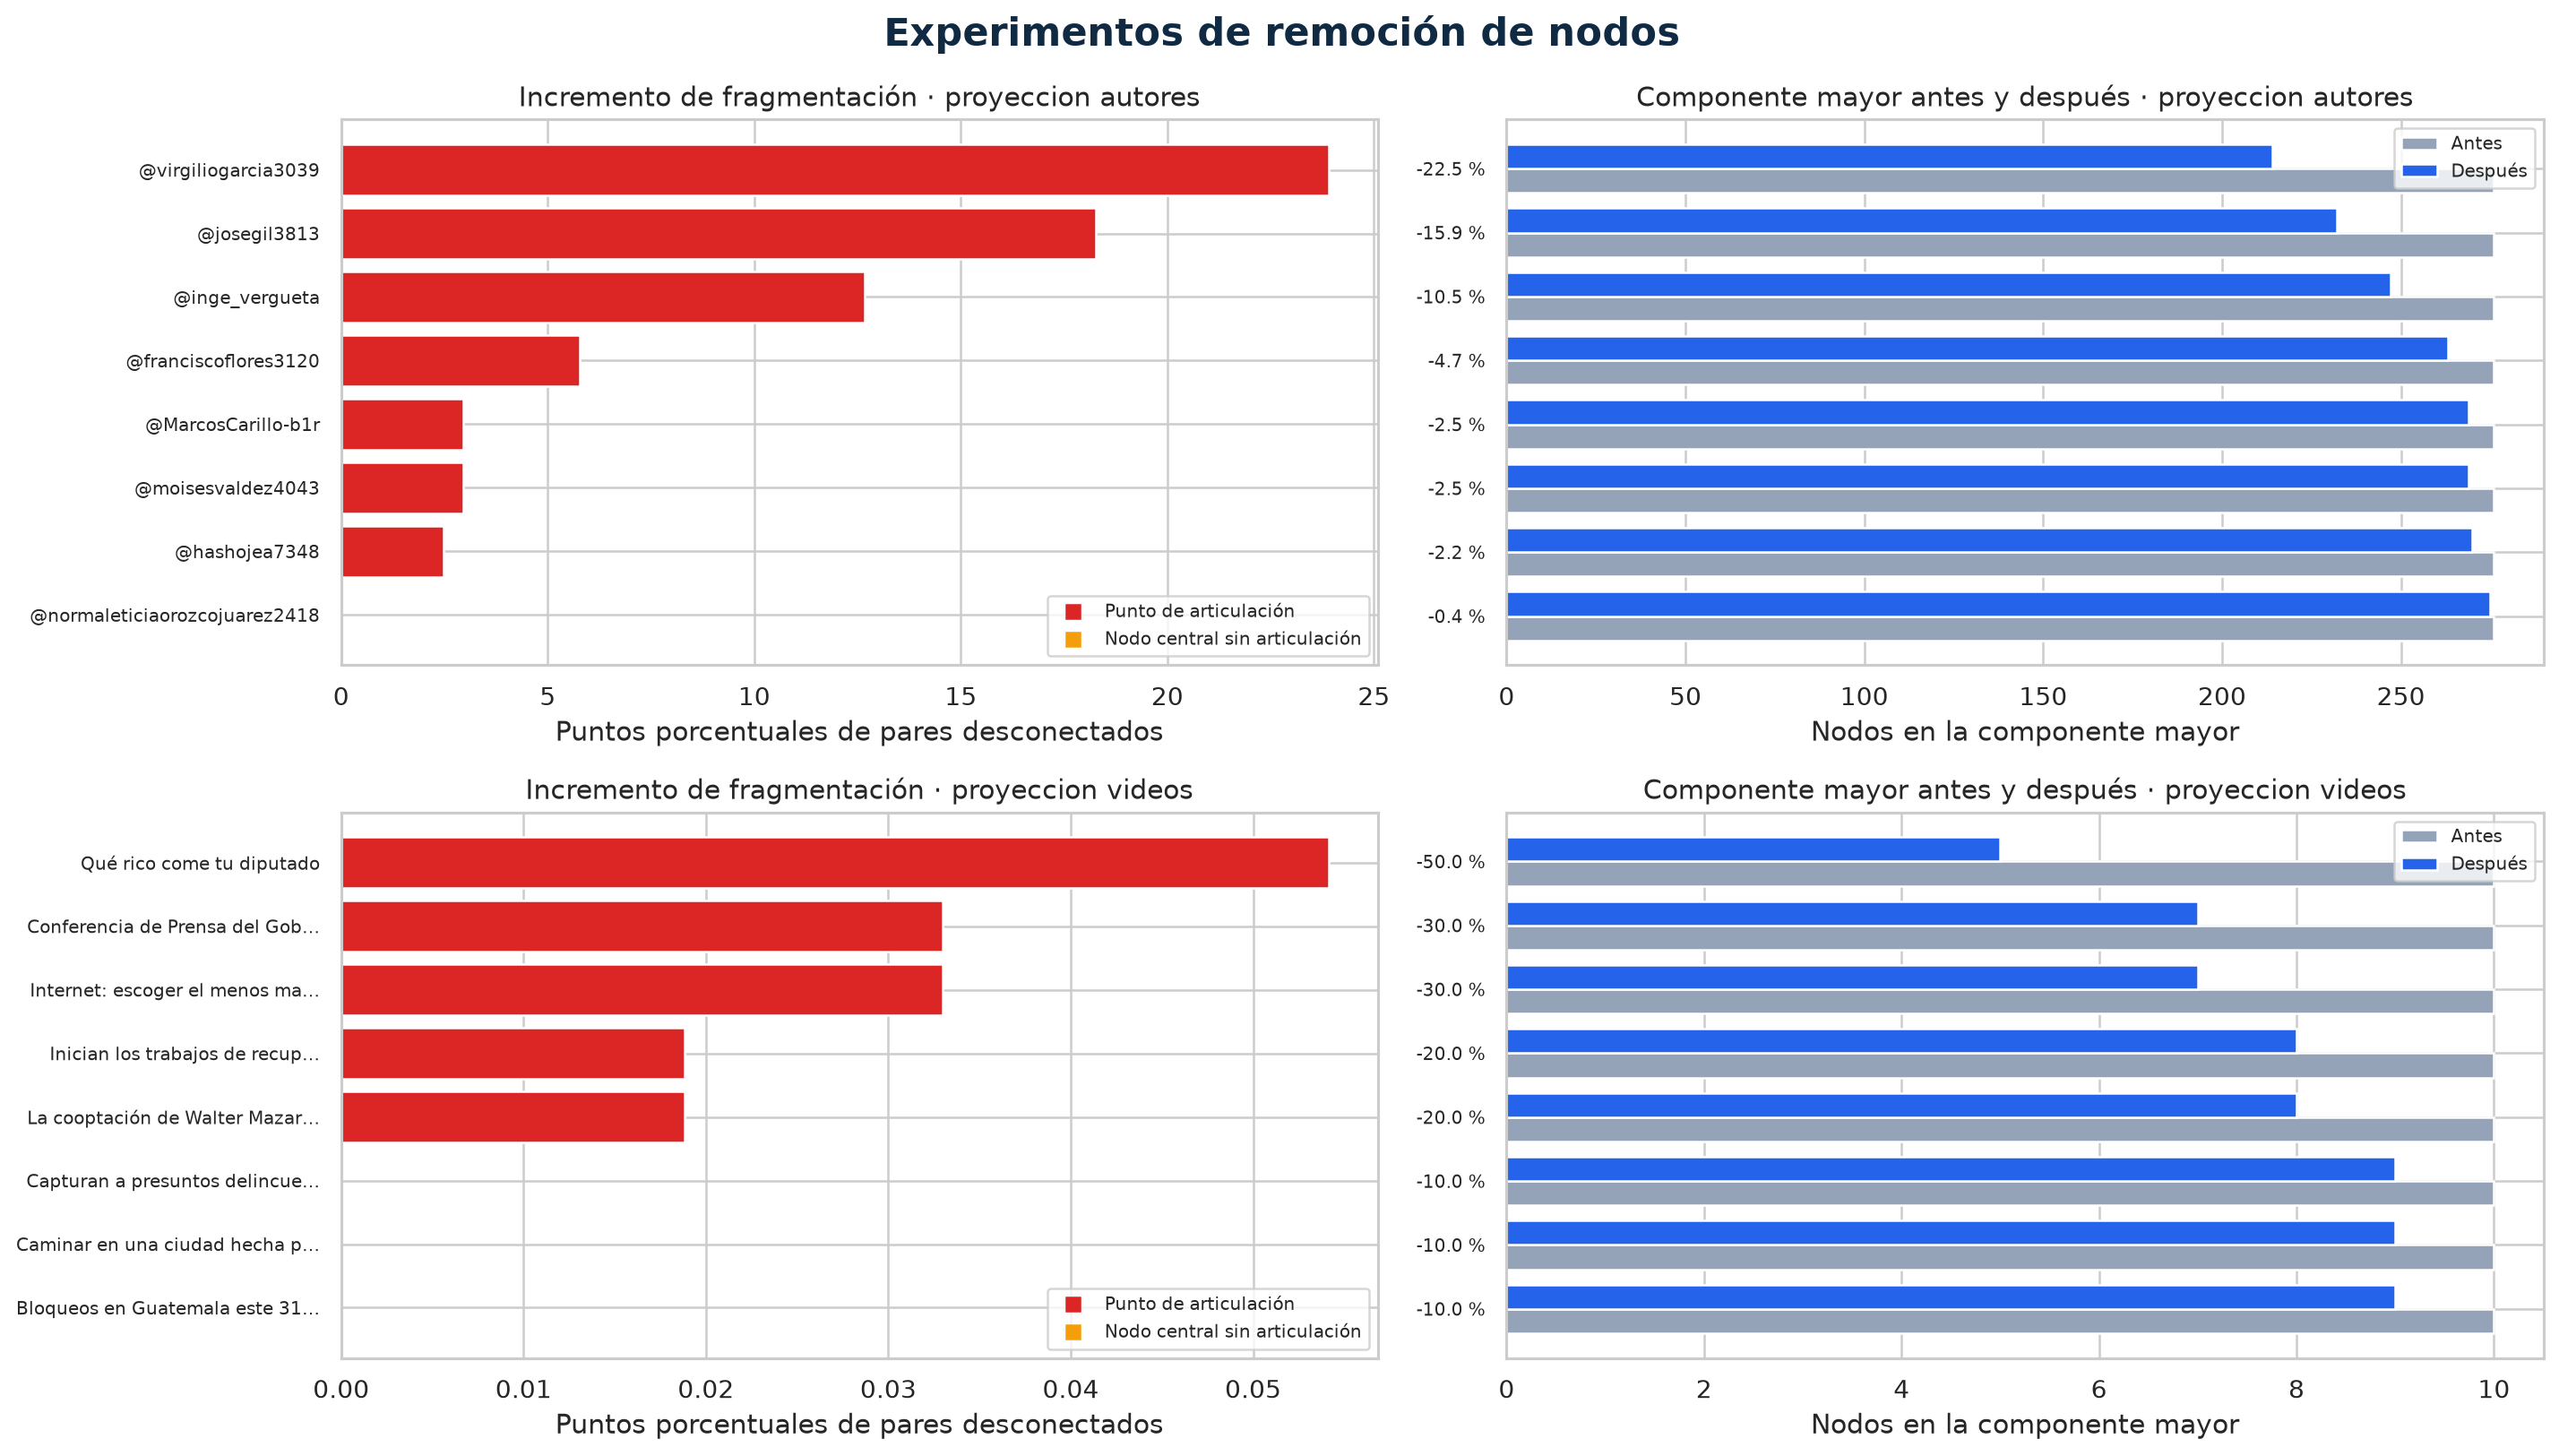
\includegraphics[width=0.9\textwidth]{impacto_remocion.png}
\caption{Impacto en la fragmentación al remover autores puente candidatos.}
\end{figure}

\section{Análisis de contenido y sentimiento}
\label{sec:sentimiento}

Se aplicó el modelo \texttt{pysentimiento/robertuito-sentiment-analysis}, especializado en sentimiento de texto social en español. El modelo conserva las probabilidades para las clases negativo, neutral y positivo, además de la confianza de cada predicción. Los resultados deben interpretarse como una clasificación automática descriptiva de esta muestra y no como una medición de la opinión de toda la audiencia.

\begin{figure}[H]
\centering
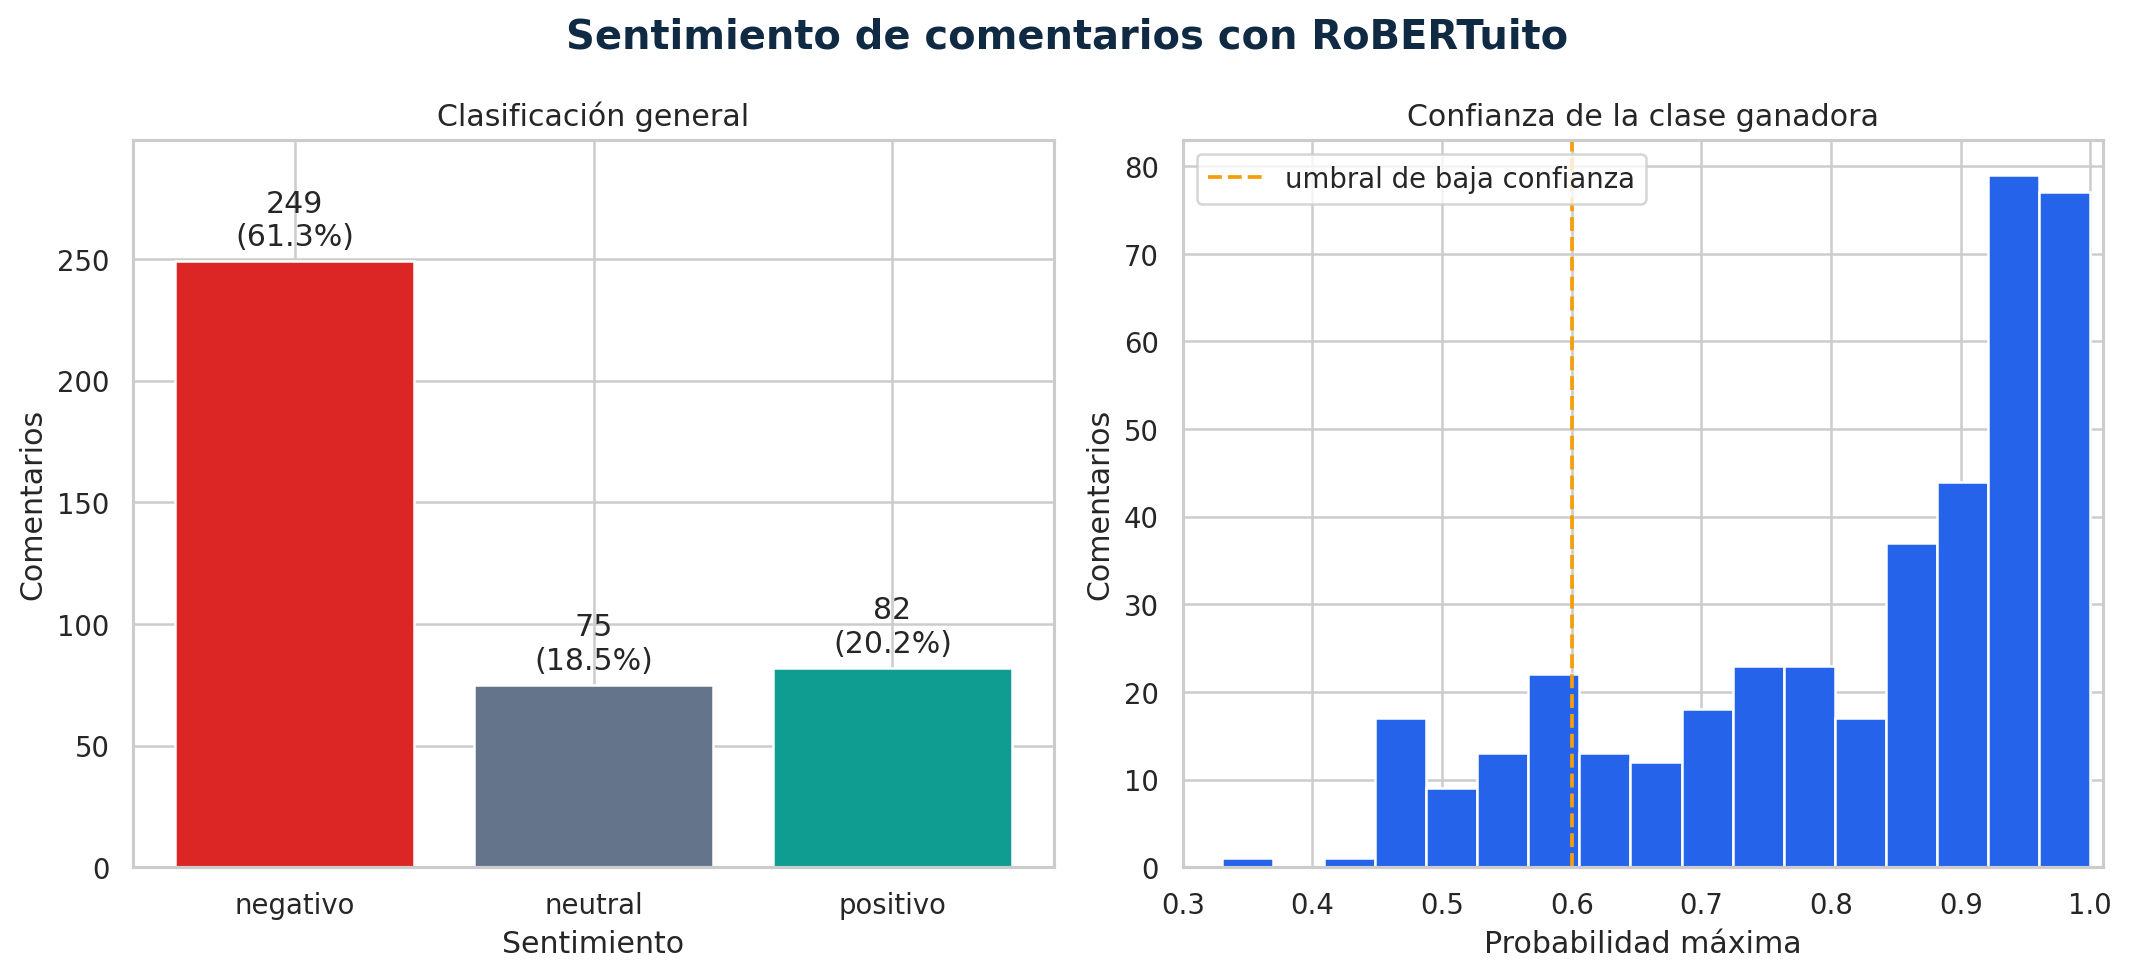
\includegraphics[width=0.98\textwidth]{sentimiento_panorama.png}
\caption{Distribución y confianza del modelo de sentimiento en los comentarios analizados.}
\end{figure}

De los 406 comentarios, 82 fueron clasificados como positivos (20.2\%), 249 como negativos (61.3\%) y 75 como neutrales (18.5\%). Predomina, por tanto, el sentimiento negativo en la muestra analizada. La confianza promedio de las predicciones fue 0.818; 61 comentarios presentaron confianza menor a 0.60 y deben interpretarse con mayor cautela. Estos resultados describen los comentarios recolectados y no permiten generalizar a toda la audiencia de YouTube.

\section{Limitaciones}

\begin{itemize}
  \item Solo 19 de 293 videos tienen comentarios, de modo que 274 aislados representan principalmente cobertura desigual.
  \item La selección por consultas y canales condiciona categorías, actores y temas visibles.
  \item \texttt{published\_time} y \texttt{published\_text} son tiempos relativos y no fechas exactas.
  \item Visualizaciones, likes y respuestas son conteos observados durante la recolección y cambian con el tiempo.
  \item No existen relaciones explícitas autor--autor ni datos sobre quién respondió a quién.
  \item La alta transitividad de la proyección de autores surge en parte de la proyección de grupos que comentan un mismo video.
  \item La concentración en pocos videos impide generalizar a todos los usuarios de YouTube o a la población de Guatemala.
\end{itemize}

Adicionalmente: solo 9 de 332 autores tienen intermediación positiva y el sentimiento se obtuvo mediante clasificación automática, por lo que las lecturas de centralidad y de sentimiento describen esta muestra acotada, no su totalidad.

Se distingue descripción de asociación e inferencia. Los conteos, la estructura de red y las proporciones de sentimiento son \textbf{descriptivos} de esta muestra. La coincidencia entre nodos de alta intermediación y videos de sentimiento más negativo es una \textbf{asociación} observada, no una relación causal probada. No se generaliza a todos los usuarios de YouTube ni a toda la población de Guatemala: la muestra fue construida por consultas específicas y cubre un periodo y conjunto de canales acotado.

\section{Interpretación y conclusiones finales}

La participación observada está altamente concentrada y la estructura de redes confirma ese patrón: la red autor--video forma grupos por video unidos por muy pocos autores puente (9 de 332), y el sentimiento negativo se concentra precisamente en el video que actúa como articulador estructural, \emph{Qué rico come tu diputado}. En este corpus específico, pocos videos concentran participación y visibilidad, mientras el resto queda fragmentado y mayormente aislado. Las diferencias de sentimiento entre contenidos son asociaciones descriptivas de la muestra y no evidencian causalidad ni un patrón general de YouTube.

La red revela \emph{quién} conecta qué contenidos; el análisis de sentimiento revela \emph{qué tono} domina esas conexiones. El modelo procesó los 406 comentarios (100\% del corpus); 61 predicciones con confianza menor a 0.60 requieren especial cautela. Ambas lecturas siguen acotadas por una cobertura parcial de videos y un muestreo por consultas. Las conclusiones se limitan a esta muestra observada y no a la totalidad de la conversación pública en YouTube sobre estos temas ni a la población general de Guatemala.

\section{Reproducibilidad}

El flujo completo se ejecuta con \texttt{python scripts/run\_final.py}; este comando genera las tablas, figuras, redes, centralidades, experimentos de remoción y resultados de sentimiento en \texttt{outputs/}. El notebook final se reconstruye con \texttt{python scripts/build\_final\_notebook.py} y, al usar \emph{Run All}, vuelve a ejecutar el mismo pipeline antes de presentar los resultados. El cargador acepta CSV real y libros Excel aunque la extensión sea incorrecta. La auditoría se ejecuta con \texttt{python scripts/audit\_final.py} y la suite de 40 pruebas con \texttt{python -m pytest -q}. Código, dependencias e instrucciones están disponibles en \repo.

\begin{thebibliography}{9}
\bibitem{networkx} Hagberg, A., Schult, D. y Swart, P. (2008). \emph{Exploring network structure, dynamics, and function using NetworkX}. Proceedings of SciPy.
\bibitem{louvain} Blondel, V., Guillaume, J., Lambiotte, R. y Lefebvre, E. (2008). \emph{Fast unfolding of communities in large networks}. Journal of Statistical Mechanics.
\bibitem{centrality} Freeman, L. (1979). \emph{Centrality in social networks: Conceptual clarification}. Social Networks, 1(3), 215--239.
\bibitem{robertuito} Pérez, J. M., Giudici, J. C. y Luque, F. (2021). \emph{pysentimiento: A Python Toolkit for Sentiment Analysis and SocialNLP Tasks}. arXiv:2106.09462. Modelo: \url{https://huggingface.co/pysentimiento/robertuito-sentiment-analysis}.
\end{thebibliography}

\end{document}
